% !TeX program = lualatex
\InputIfFileExists{blueprint-local-fonts.tex}{}{}
\documentclass[a4paper,10pt]{ltjsarticle}
\usepackage[margin=23mm,headheight=16pt]{geometry}
\usepackage{amsmath,amssymb,amsthm,mathtools}
\usepackage{expl3,graphicx,booktabs,longtable,array,seqsplit}
\usepackage{xcolor,fancyhdr,enumitem}
\usepackage[unicode,colorlinks=true,linkcolor=blue!50!black,urlcolor=blue!50!black]{hyperref}
\newcommand{\Z}{\mathbb Z}
\newcommand{\Q}{\mathbb Q}
\newcommand{\R}{\mathbb R}
\newcommand{\N}{\mathbb N}
\newcommand{\Sol}{\mathcal S}
\newcommand{\Reach}{\operatorname{Reach}}
\newcommand{\Latt}{\operatorname{Latt}}
\newcommand{\F}{F}
\newtheorem{theorem}{定理}[section]
\newtheorem{proposition}[theorem]{命題}
\newtheorem{lemma}[theorem]{補題}
\newtheorem{corollary}[theorem]{系}
\theoremstyle{definition}
\newtheorem{definition}[theorem]{定義}
\newtheorem{example}[theorem]{例}
\theoremstyle{remark}
\newtheorem{remark}[theorem]{注意}
\renewcommand{\proofname}{証明}

\newcommand{\leanok}{}
\newcommand{\notready}{}
\newcommand{\mathlibok}{}
\newcommand{\discussion}[1]{}
\ExplSyntaxOn
\NewDocumentCommand{\code}{m}{\texttt{
  \seq_set_split:Nnn \l_tmpa_seq { ~ } {#1}
  \seq_map_indexed_inline:Nn \l_tmpa_seq {
    \int_compare:nNnT {##1} > {1} {\space}
    \seqsplit{##2}
  }
}}
\NewDocumentCommand{\lean}{m}{
  \leavevmode\par\smallskip
  {\footnotesize\normalfont\sffamily
   \clist_map_inline:nn{#1}{\noindent Lean:~\nolinkurl{##1}\par}}
  \smallskip
}
\NewDocumentCommand{\uses}{m}{\clist_map_inline:nn{#1}{\vphantom{\ref{##1}}}\ignorespaces}
\NewDocumentCommand{\proves}{m}{\clist_map_inline:nn{#1}{\vphantom{\ref{##1}}}\ignorespaces}
\ExplSyntaxOff
\newcommand{\depview}{\begin{center}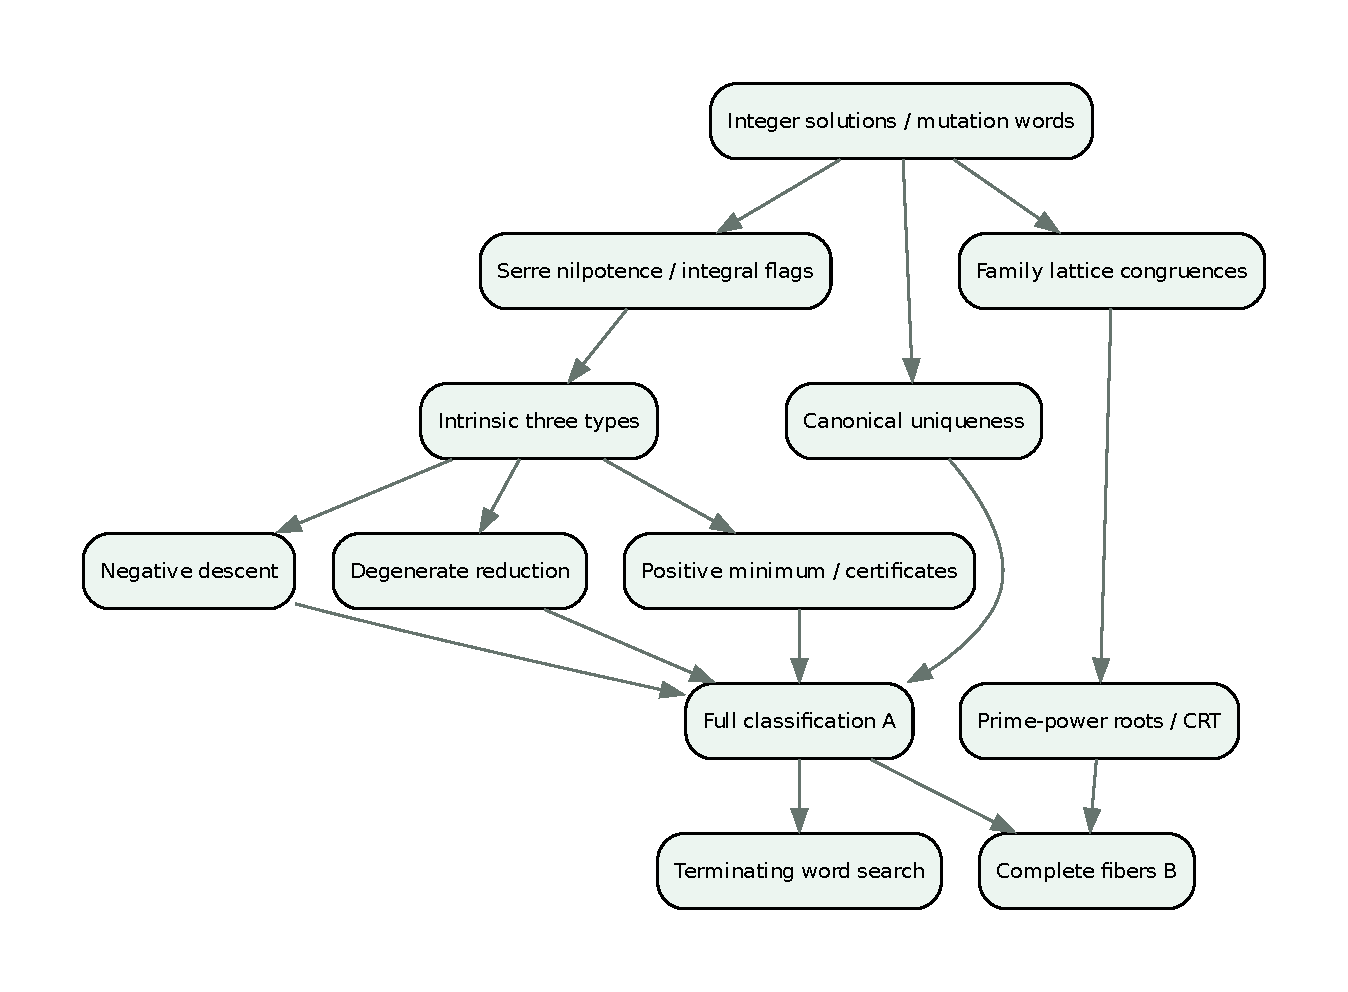
\includegraphics[width=0.91\textwidth]{overview.pdf}\end{center}}

\setlength{\emergencystretch}{3em}
\setlength{\parskip}{0.15em}
\allowdisplaybreaks[2]
\raggedbottom
\pagestyle{fancy}\fancyhf{}
\fancyhead[L]{\small Serre--Markov Lean Blueprint}
\fancyhead[R]{\small 数学と形式化の対応}
\fancyfoot[C]{\thepage}
\setcounter{tocdepth}{2}
\title{Serre--Markov 分類の Lean Blueprint\\\large 定義・証明経路・依存関係と検証済みコード}
\author{植田 一石 (Kazushi Ueda)}
\date{2026年10月5日}
\begin{document}
\maketitle
\section*{この Blueprint の読み方}
本書は、三次元型 Serre 格子の整数 Gram 行列を分類する Lean プロジェクトの設計と証明を解説する。
対象は2026年10月4日の日本語原稿 v4である。主分類、格子同型類への忘却写像のファイバー、
停止する判定手続きの結論は形式化済みである。証明経路は、原稿の双曲幾何による経路をそのまま移植するのではなく、
整数下降、反射語の代数、最小高さ、多項式非負証明書を使って構成した。

各定義・定理の Lean 対応には完全修飾した宣言名を付ける。HTML版のチェック印は、対応する定義または定理と証明が
形式化済みであることを表す。これは本文の自然言語説明を別途機械検証したという意味ではない。
依存グラフの辺は、本書で明示した数学的依存であり、コンパイラが生成する全補助宣言の依存ではない。
コードの厳密な内容を確認する場合は、各宣言リンクと検証ログを参照する。

基礎体や抽象圏を入力には取らない。分類対象は六つの整数と、それらを Gram 成分とする階数4の Euler 格子である。
したがって、固定した三角圏の例外列の推移性や、X72 の三次元幾何的実現を結論する文書ではない。

\subsection*{主な到達点}
任意の解は、正規化した負側の族 $\F(x,y)$（$x\ge y\ge0$、$x+y>0$）、
退化族 $\F(k,-k)$（$k\ge0$）、五つの正側代表のうちちょうど一つに到達する。
同じ整数格子に属する軌道の全ファイバーは有限であるが、その大きさには一様な上界がない。
同値であるかどうかを判定し、同値な場合に実際の変異語を返す停止算法も証明済みである。
全体を読み始めるときは、基本設定から三型の分離、次に負側・退化型と正側の存在・一意性、
最後にファイバーと算法の順に読むとよい。

\depview
\tableofcontents
\section{基本設定と内在的な三型}
\subsection{六成分・変異語・二つの同値関係}
\begin{definition}[整数六つ組と Gram 行列]\label{bp:def-six}
\lean{SerreMarkov.Six,SerreMarkov.gram,SerreMarkov.gramInverse}\leanok
整数六つ組 $z=(a,b,c,d,e,f)$ に対して
\[
M(z)=\begin{pmatrix}1&a&b&c\\0&1&d&e\\0&0&1&f\\0&0&0&1\end{pmatrix},
\qquad \chi_z(x,y)=x^{\mathsf T}M(z)y
\]
と定める。格子の台は $\Z^4$ であり、$\chi_z$ は対称とは限らない。
\end{definition}
Lean の行列型は $\operatorname{Matrix}(\operatorname{Fin}4,\operatorname{Fin}4,\Z)$、
六成分は名前付きの構造体である。基底添字は0から3までである。
上三角対角成分1を型で固定することで、後の計算に可逆性の仮定を繰り返し付ける必要をなくしている。
整数逆行列は一般の逆行列計算に委ねず、成分が整数多項式である具体式として最初に与える。

\begin{definition}[二方程式の解]\label{bp:def-solution}
\lean{SerreMarkov.q1,SerreMarkov.q2,SerreMarkov.isSolution,SerreMarkov.Solution}\leanok
\uses{bp:def-six}
\begin{align*}
q_1(z)&=acdf-abd-ace-bcf-def+a^2+b^2+c^2+d^2+e^2+f^2,\\
q_2(z)&=af-be+cd,\\
\Sol&=\{z\in\Z^6:q_1(z)=8,\ q_2(z)^2=16\}.
\end{align*}
証明付き入力型は $\{z:\Z^6\mid z\in\Sol\}$ である。
\end{definition}
$q_2=4$ と $q_2=-4$ を最初から両方含める。符号変更は $q_2$ の符号を反転することがあるため、
保存される方程式は平方を取ったものである。この規約は有限列挙と一般分類のどちらにも一貫して用いる。

\begin{definition}[実際の有限変異語]\label{bp:def-reachable}
\lean{SerreMarkov.Generator,SerreMarkov.step,SerreMarkov.applyWord,SerreMarkov.Reachable}\leanok
\uses{bp:def-six}
生成子は三つの変異、その三つの逆、四つの基底符号変更の合計10個である。
例えば
\[
\sigma_1(a,b,c,d,e,f)=(a,ab-d,ac-e,b,c,f).
\]
語 $w=[g_1,\ldots,g_n]$ は $g_1$ から順に作用させる。
$\Reach(z,z')$ は、有限語 $w$ が存在して $w\cdot z=z'$ となることである。
\end{definition}
語はリストにより実装される。任意置換、格子同型、逆順化を生成子として追加していない。
後で補助的に逆順化を用いる場合にも、元の同値関係に操作を追加してよいかどうかを個別に証明する。

\begin{lemma}[方程式の保存と可逆性]\label{bp:mutation-invariants}
\lean{SerreMarkov.applyWord_preserves_solution,SerreMarkov.applyWord_inverse,SerreMarkov.reachable_equivalence,SerreMarkov.braid12,SerreMarkov.braid23,SerreMarkov.braid13}\leanok
\uses{bp:def-solution,bp:def-reachable}
各生成子は解集合を保存する。逆生成子を逆順に並べた語は元の語の作用を取り消す。
従って $\Reach$ は同値関係であり、三変異は $B_4$ の組み紐関係を満たす。
\end{lemma}
\begin{proof}\leanok\uses{bp:def-reachable,bp:def-solution}
六成分の各等式を成分ごとに展開し、整数多項式の恒等式として示す。
基本の保存式は $q_1(\sigma_i z)=q_1(z)$ と $q_2(\sigma_i z)=q_2(z)$、
符号変更については $q_2(\varepsilon_i z)=-q_2(z)$ である。
リストに関する帰納法で任意長の語へ延長する。Lean では構造体の外延性、
簡約、可換環の正規化を組み合わせる。有限範囲の整数検査ではない。
\end{proof}

\begin{definition}[整数 Euler 格子同型]\label{bp:def-lattice}
\lean{SerreMarkov.LatticeEquivalent,SerreMarkov.latticeSetoid,SerreMarkov.solutionSetoid,SerreMarkov.solutionForgetfulMap}\leanok
\uses{bp:def-six,bp:def-reachable,bp:def-solution}
$\Latt(z,z')$ を、整数可逆行列 $B\in\operatorname{GL}_4(\Z)$ が存在して
$B^{\mathsf T}M(z)B=M(z')$ となることと定める。解軌道の商から格子同型類の商への写像を
\[
\pi:\Sol/{\Reach}\longrightarrow\Z^6/{\Latt},\qquad [z]\longmapsto[z]
\]
と書く。右辺は全六つ組の格子同型商であり、像にないクラスのファイバーは空である。
\end{definition}
Lean では整数行列環の unit を量化する。これにより、行列式非零という有理可逆性と、
行列式 $\pm1$ という整数可逆性を取り違えない。商を使うときは、各写像が同値関係を保存することを
明示的に渡して定義する。

\begin{proposition}[語から整数基底変更へ]\label{bp:basis-congruence}
\lean{SerreMarkov.reachable_integral_congruence,SerreMarkov.reachable_latticeEquivalent}\leanok
\uses{bp:def-lattice,bp:mutation-invariants}
$\Reach(z,z')$ なら $\Latt(z,z')$ である。実際、到達語から行列式 $\pm1$ の整数基底変更行列を構成できる。
\end{proposition}
\begin{proof}\leanok\uses{bp:def-reachable,bp:def-six}
一生成子に対応する基底変更を行列として与え、その合同式を直接計算する。
語に沿ってこれらを掛け、行列式の積と合同式を帰納法で追う。
この命題によって忘却写像は well-defined になる。一方、逆向きは一般には成立しない。
同じ格子に複数の変異軌道があることは、後のファイバー定理の主題である。
\end{proof}

\begin{definition}[Serre 作用素と三次の判定量]\label{bp:def-serre}
\lean{SerreMarkov.serre,SerreMarkov.shiftedSerre,SerreMarkov.symmetricForm,SerreMarkov.IntrinsicSigns.thirdMinorSum}\leanok
\uses{bp:def-six}
\[
S=M^{-1}M^{\mathsf T},\qquad N=S+I,\qquad H=M+M^{\mathsf T}.
\]
$T(z)$ を $H$ の四つの主三次小行列式の和とする。
\end{definition}
ここでは $S$ を $M^{-1}M^{\mathsf T}$ と定義する。別の文献で使われる $-S$ と混同すると、
三次元型の固有値規約が反転する。本プロジェクトの三次元型は $N^4=0$、すなわち $S$ の固有値がすべて $-1$ の場合である。

\begin{theorem}[二方程式と四乗零の同値]\label{bp:matrix-nilpotent}
\lean{SerreMarkov.solution_iff_fourth_power_zero}\leanok
\uses{bp:def-solution,bp:def-serre}
任意の整数六つ組について $z\in\Sol$ と $N(z)^4=0$ は同値である。
\end{theorem}
\begin{proof}\leanok\uses{bp:def-six,bp:def-serre,bp:def-solution}
具体的な整数逆行列から $N$ の特性多項式を計算する。
二方程式を代入すると特性多項式は $X^4$ となり、Cayley--Hamilton の定理から $N^4=0$ を得る。
逆に $N^4=0$ ならば $N$ は冪零なので、その特性多項式は $X^4$ である。
計算済みの特性多項式の三次係数と定数項を比較すると二方程式が従う。
具体的な行列計算と一般の特性多項式の定理を組み合わせ、
固有値や Jordan 標準形を個別に構成する必要をなくしている。
\end{proof}

\begin{definition}[基本族]\label{bp:def-family}
\lean{SerreMarkov.family,SerreMarkov.family_isSolution}\leanok
\uses{bp:def-solution}
\[
\F(x,y)=(-x,-x,-2,2,-y,-y),\qquad x,y\in\Z.
\]
任意のパラメータで $\F(x,y)\in\Sol$ である。
\end{definition}
\begin{proof}\leanok\uses{bp:def-solution}
二方程式へ代入すると $q_1=8$、$q_2=-4$ が整数多項式恒等式として得られる。
\end{proof}
\begin{definition}[整数下降に用いる高さ]\label{bp:def-height}
\lean{SerreMarkov.NegativeDescent.l1,SerreMarkov.NegativeDescent.integerL1}\leanok
\uses{bp:def-six}
$h(z)=|a|+|b|+|c|+|d|+|e|+|f|\in\N$ とする。
自然数値の高さと、同じ式を整数値に取ったものを別に定義し、両者が一致することを示す。
\end{definition}
自然数型の高さは強帰納法に、整数型の式は不等式・多項式の正規化に使う。
絶対値を含む式を一度に正規化せず、符号別に扱うことが境界分割の設計上重要である。

\subsection{原始旗・適合基底・内在的な符号}
\begin{theorem}[正則解の原始整数旗と適合基底]\label{bp:intrinsic-frame}
\lean{SerreMarkov.solution_regular_has_primitive_flag,SerreMarkov.IntrinsicFrame.solution_regular_has_frame,SerreMarkov.IntrinsicFrame.frame_gram,SerreMarkov.IntrinsicFrame.frame_determinant}\leanok
\uses{bp:matrix-nilpotent,bp:def-lattice}
$z\in\Sol$、$N^3\ne0$ とする。原始整数ベクトル $p,\ell$ と正整数 $\kappa$ を取り、
$Np=0$、$N\ell=-\kappa p$、$\ker N=\Z p$、$\ker N^2=\Z p+\Z\ell$ とできる。
座標 $r(x)=\chi(x,p)$、$d(x)=\chi(x,\ell)$ は組として $\Z^2$ へ全射である。
その全射性から得る $u,v$ を用い、基底 $(u,v,\ell,p)$ の Euler 行列は
\[
E=\begin{pmatrix}
\alpha&\beta&0&1\\
\gamma&-A&1&0\\
-\kappa&-1&0&0\\
-1&0&0&0
\end{pmatrix}
\]
となる。基底変更行列の行列式は $\pm1$ である。
\end{theorem}
\begin{proof}\leanok\uses{bp:matrix-nilpotent,bp:def-lattice}
まず有理数上で nilpotent 作用素の核と像の次元を計算する。
整数核は自由加群内の飽和部分加群となるので、原始生成元と分裂を整数上へ戻す。
原始的な二座標の全射性を証明し、像 $(1,0),(0,1)$ の逆像から $u,v$ を選ぶ。
Euler 対の必要な成分を Serre 関係から導いて $E$ を得る。
最後に $\det M=\det E=1$ を使うと、基底変更行列 $B$ について $\det(B)^2=1$ となる。
単に有理基底が得られた段階で整数基底と呼ばないことが、この部分の形式化の要点である。
\end{proof}

\begin{proposition}[立方テンソル、content、Riemann--Roch 恒等式]\label{bp:intrinsic-formula}
\lean{SerreMarkov.IntrinsicFrame.frame_cube_action,SerreMarkov.IntrinsicFrame.frame_cube_content,SerreMarkov.IntrinsicFrame.frame_RiemannRoch}\leanok
\uses{bp:intrinsic-frame}
任意の $x$ に対して $N^3x=2A\kappa^2r(x)p$ であり、$N^3$ の整数成分の content は $2|A|\kappa^2$ である。
$\chi(x,x)=\chi(y,y)=1$ なら
\[
(\chi(x,y)+\chi(y,x))r(x)r(y)
=r(x)^2+r(y)^2+A\bigl(r(x)d(y)-r(y)d(x)\bigr)^2.
\]
\end{proposition}
\begin{proof}\leanok\uses{bp:intrinsic-frame}
適合基底での $N^3$ は一つの成分だけが $2A\kappa^2$ で、他は零である。
整数可逆合同・共役に対する content の不変性から元の基底の式へ移す。
RR式では $q=r(y)x-r(x)y$ を取り、$r(q)=0$ を使う。
rank核上の対称対は $-2A\,d(q)^2$ なので、$\chi(q,q)$ の展開と比較して式が得られる。
幾何的な Riemann--Roch 定理や正階数の仮定はこの恒等式の証明には不要である。
\end{proof}

\begin{theorem}[内在量と三型の分離]\label{bp:intrinsic-kind}
\lean{SerreMarkov.IntrinsicUnique.solution_regular_unique_parameters,SerreMarkov.IntrinsicUnique.latticeEquivalent_frame_invariants,SerreMarkov.intrinsicKind,SerreMarkov.latticeEquivalent_intrinsicKind,SerreMarkov.solution_cube_zero_iff_thirdMinorSum_zero}\leanok
\uses{bp:intrinsic-frame,bp:intrinsic-formula,bp:def-serre}
正則解の $(A,\kappa)$ は旗・適合基底の選択に依存せず、整数 Euler 格子同型で保存される。
$N^3=0$ と $T=0$ は同値であり、$N^3\ne0$ のとき $T$ の符号は $A$ の符号に一致する。
従って解を退化型 $N^3=0$、正側 $T>0$、負側 $T<0$ に重複なく分けられ、
その型は格子同型と変異で保存される。
\end{theorem}
\begin{proof}\leanok\uses{bp:intrinsic-frame,bp:intrinsic-formula,bp:basis-congruence}
二つの原始旗では $p$ の生成元の違いは $\pm1$、$\ell$ の差は $p$ の整数倍と生成元の符号だけである。
座標の全射性と $\kappa>0$ により $\kappa$ が一致し、rank核上の対称形式から $A$ も一致する。
対称行列の余因子を $2A\kappa^2pp^{\mathsf T}$ と書けば、主余因子の和の符号が決まる。
分類に入る前にこれらを証明するため、分類を使って分類の型不変性を証明する循環は生じない。
\end{proof}

\begin{proposition}[実対角合同による符号の証明証書]\label{bp:intrinsic-diagonal}
\lean{SerreMarkov.IntrinsicSignature.real_frame_diagonal_congruence,SerreMarkov.IntrinsicSignature.realFrameChange_isUnit}\leanok
\uses{bp:intrinsic-frame,bp:intrinsic-kind}
正則解の $H$ は実可逆合同により $\operatorname{diag}(2,-2,-2A,0)$ へ移る。
\end{proposition}
\begin{proof}\leanok\uses{bp:intrinsic-frame}
適合行列から有理係数の具体的な可逆行列を構成し、合同式を成分計算する。
実数への係数写像で同じ式が得られる。本実装の符号数は、この表示された対角成分の符号を数えた証明証書である。
任意の実行列について慣性指数を定義して一般の Sylvester 理論を展開したAPIとは区別する。
\end{proof}

\begin{proposition}[実基底変異と反射 Hurwitz 操作]\label{bp:reflection-hurwitz}
\lean{SerreMarkov.basisWord_reflection_hurwitz,SerreMarkov.ReflectionGroup.reachable_reflectionGroup_isometric_conjugate}\leanok
\uses{bp:basis-congruence,bp:def-serre}
基底元による四反射は任意の実変異語に対し Hurwitz 操作を受ける。
従って、それらが生成する実際の整数反射部分群は変異に沿って整数等長共役となる。
\end{proposition}
\begin{proof}\leanok\uses{bp:basis-congruence,bp:def-reachable}
一生成子の更新式を行列積として比較し、任意長の語に対し帰納する。
符号変更は旧座標での反射を変えない。後の family 一意性では、抽象的な反射ラベルだけでなく、
この実整数表現との接続を使う。Coxeter群の一般的な Hurwitz 推移性定理を仮定する命題ではない。
\end{proof}

\section{負側と退化型の分類}

この章は、整数解を標準代表へ移す存在証明と、標準代表どうしを分離する
一意性証明を扱う。両者は異なる問題である。存在には高さに関する整礎帰納法を
用い、一意性には整数反射語と境界の合同不変集合を用いる。原稿の双曲反射群の
基本領域からの証明を形式化したものではなく、実装された代数的証明の依存関係を
示す。

以下、\(G_z\) はEuler行列、\(H_z=G_z+G_z^{\mathsf T}\) はその対称化、
\(N_z=G_z^{-1}G_z^{\mathsf T}+I\) はシフトしたSerre作用素とする。
\(\tau(z)\) は \(H_z\) の四つの主三次小行列式の和である。
負側は \(\tau(z)<0\)、退化側は \(N_z^3=0\) で特徴付けられる。
\(\Reach(z,w)\) は符号変更も許した有限の変異語による到達可能性を表す。
整数格子の同型条件 \(\Latt(z,w)\) とは、ある \(B\in GL_4(\Z)\) に対する
\(B^{\mathsf T}G_zB=G_w\) である。

\subsection{退化型をCayley立方へ移す}

退化型を先に扱うと、分類に使う整数的な降下の仕組みが三変数で見える。
四次の冪零性だけからは、一般の行列について \(N^3=0\) と \(N^2=0\) は同値で
ない。この問題ではEuler行列の特別な形と二つの解方程式を合わせることで、
Jordan型 \([3,1]\) が除外される。

\begin{proposition}[退化型の整数正規表示]
\label{bp:deg-reduced}
\lean{SerreMarkov.cofactor_zero_of_cube_zero}
\lean{SerreMarkov.cofactor_zero_reduced}
\lean{SerreMarkov.cube_zero_implies_square_zero}
\leanok
\(z\in\Sol\) かつ \(N_z^3=0\) とする。このとき \(N_z^2=0\) である。
さらに、一つの符号変更で \(q_2(z)=-4\) にそろえれば、
\[
 z=D(a,b,d):=(a,b,-d,d,b-ad,-a),
 \qquad a^2+b^2+d^2-abd=4
\]
という整数表示を得る。符号変更が不要な場合はもとの解自身がこの表示を持つ。
\end{proposition}
\begin{proof}
\uses{bp:def-solution,bp:matrix-nilpotent}
\leanok
解方程式から \(q_2(z)^2=16\) である。第一基底ベクトルの符号変更は
\(q_2\) の符号を反転させ、\(N_z\) を整数対角行列による共役へ移す。
したがって、三乗零を保ったまま \(q_2=-4\) としてよい。

\(\det(tI-N_z)=t^4\) と \(N_z^3=0\) から
\[
 \operatorname{adj}(tI-N_z)=t^3I+t^2N_z+tN_z^2
\]
を多項式行列として証明する。右辺と \(tI-N_z\) の積は \(t^4I\) である。
左辺にも同じ積公式があり、非零の行列式を持つ多項式行列の右消去によって両者が
一致する。\(t=0\) の評価で \(\operatorname{adj}(N_z)=0\) を得る。
\(H_z=G_zN_z\) なので \(\operatorname{adj}(H_z)=0\) でもある。

ここから三つの平方和の恒等式を使う。第一の恒等式は
\(8(a+f)^2\)、第二は \(8(c+d)^2\) を、対称余因子と \(q_2+4\) の
整数多項式結合として表す。これらを零とすれば \(f=-a\)、\(c=-d\) となる。
第三の恒等式は、その代入後の \(2(b-e-ad)^2\) を同じように表すため、
\(e=b-ad\) が従う。したがって \(z=D(a,b,d)\) であり、
\[
 q_2(D(a,b,d))=-(a^2+b^2+d^2-abd)
\]
がCayley立方の方程式を与える。

最後に、\(N_{D(a,b,d)}^2\) の十六成分を計算すると、すべてが
\(q_2(D(a,b,d))+4\) を因子に持つ。これが零なので二乗零である。
実装では多項式恒等式を \code{ring}、平方の非負性を明示した算術推論を
\code{nlinarith} で検査する。随伴行列の消滅から出発しており、退化型の分類を
先に仮定していない。
\end{proof}

\begin{lemma}[Cayley立方の整数Vieta降下]
\label{bp:deg-vieta}
\lean{SerreMarkov.markov_sign_normalized_cases}
\lean{SerreMarkov.markov_positive_descent}
\leanok
整数 \(a,b,d\) が \(a^2+b^2+d^2-abd=4\) を満たすとする。
偶数個の符号変更で \(a,b\ge0\) にそろえると、次のいずれかが成立する。
\[
 |a|=2\ \text{または}\ |b|=2\ \text{または}\ |d|=2;
 \qquad (a,b,d)=(1,1,-1);
 \qquad a,b,d\ge3.
\]
最後の場合、巡回置換で \(d\ge a,b\) とすれば
\[
 0<ab-d<d.
\]
したがってVieta変換 \(d\mapsto ab-d\) は三変数の絶対値の和を厳密に減らす。
\end{lemma}
\begin{proof}
\uses{bp:deg-reduced}
\leanok
\(d<0\) の場合は \(abd\le0\) なので
\(a^2+b^2+d^2\le4\) であり、小さい整数の有限の場合分けに帰着する。
\(d\ge0\) の場合は、まず絶対値 \(2\) の座標がある分岐を取り除く。
そのうえで、どれかが \(3\) 未満ならば、その座標は \(0\) または \(1\) である。
方程式と平方の非負性によって残りの座標を有界にでき、再び絶対値 \(2\) の座標が
必要となるため矛盾する。絶対値 \(2\) の分岐ではほかの座標は有界とは限らず、
例えば \((2,b,b)\) は任意の整数 \(b\) に対する解である。
こうして任意の整数解から三つの分岐を導き、最初から有界解だけに制限しない。

大きい分岐では、さらに \(a\le b\le d\) としてよい。
\[
 d(ab-d)=a^2+b^2-4>0
\]
から新しい根の正値性を得る。一方、
\[
 (d-b)(ab-d-b)=a^2+(2-a)b^2-4<0
\]
であり、\(d-b\ge0\) なので \(ab-d<b\le d\) となる。
二つの小さい座標の順序が逆の場合は同じ議論で交換する。
積の符号を明示することで、Leanは順序体を導入せず、\(\Z\) 上の不等式として
この降下を検証する。
\end{proof}

\begin{theorem}[退化型の標準族への到達]
\label{bp:deg-surjective}
\lean{SerreMarkov.reducedDegenerate_reachable_family}
\lean{SerreMarkov.degenerate_classification_surjective}
\leanok
任意の \(z\in\Sol\) について、\(N_z^3=0\) ならば
\[
 \exists k\in\Z_{\ge0},\qquad \Reach(z,\F(k,-k))
\]
である。
\end{theorem}
\begin{proof}
\uses{bp:deg-reduced,bp:deg-vieta,bp:def-reachable,bp:def-family}
\leanok
三変数表示には、もとの変異の具体的な公式がある。
\[
 \mu_1D(a,b,d)=D(a,ab-d,b),\qquad
 \mu_2D(a,b,d)=D(ad-b,a,d).
\]
さらに \(\mu_1\) の後に \(\mu_2\) を作用させる語は
\(D(a,b,d)\mapsto D(d,a,b)\) という巡回置換になる。
二個の基底符号を変更する語は
\((a,b,d)\mapsto(-a,b,-d)\) と
\((a,b,d)\mapsto(a,-b,-d)\) を実現する。
以上はすべて、三変数の任意の整数値についての六成分恒等式である。

\(|a|+|b|+|d|\) に関する強帰納法を行う。
補題\ref{bp:deg-vieta}の大きい分岐では、上の実際の変異が高さを減らすので
帰納法の仮定を適用できる。
\(d=2\) の分岐では方程式が \((a-b)^2=0\) となり、
\(D(a,a,2)=\F(-a,a)\) である。他の位置の \(\pm2\) は符号変更と巡回置換で
この分岐へ移す。残る \((1,1,-1)\) は一回の変異で \((1,2,1)\) となり、
絶対値 \(2\) の分岐に入る。最後に同時符号反転で \(k\ge0\) にそろえる。

Leanでの到達可能性の証人は有限リストであり、帰納法の各段階で語を連結する。
抽象的な同値関係に代表が存在するだけでなく、使った各操作が実際の変異生成元で
あることまで証明される。
\end{proof}

\begin{lemma}[退化パラメータの格子不変量]
\label{bp:deg-content}
\lean{SerreMarkov.latticeEquivalent_minorDvd}
\lean{SerreMarkov.degenerate_family_minorDvd}
\lean{SerreMarkov.degenerate_family_lattice_injective}
\leanok
\uses{bp:def-family,bp:def-lattice}
対称行列のすべての二次小行列式を割る整数の集合は、整数格子同型で保存される。
\(\F(k,-k)\) についてこの集合は
\[
 \{d\in\Z:d\mid4-k^2\}
\]
である。したがって、\(k,l\ge0\) かつ
\(\Latt(\F(k,-k),\F(l,-l))\) ならば \(k=l\) である。
\end{lemma}
\begin{proof}
\uses{bp:def-family,bp:def-reachable}
\leanok
二次小行列式を
\(A_{ik}A_{jl}-A_{il}A_{jk}\) と定義する。積 \(BA\) のこの式を展開すると
\(A\) の二次小行列式の整数係数和になる。右乗法も同様であり、
合同 \(B^{\mathsf T}AB\) に対して整除性が保存される。
格子同型の逆を使うことで両方向の保存則が得られる。
Smith標準形の存在やその算法はここでは必要ない。

族の対称行列を直接代入すると、各小行列式は \(0\) または \(\pm(4-k^2)\) であり、
その一つは \(4-k^2\) そのものである。従って同型なら
\(|4-k^2|=|4-l^2|\) となる。同符号の分岐では \(k^2=l^2\) なので
非負性から \(k=l\) である。逆符号の分岐では \(k^2+l^2=8\) となり、
\(0\le k,l\le2\) に帰着して、やはり \(k=l=2\) を得る。
特に \(k=2\) の小行列式がすべて零になる境界も含まれる。
\end{proof}

\begin{theorem}[退化側の完全分類]
\label{bp:deg-classification}
\lean{SerreMarkov.degenerate_classification}
\lean{SerreMarkov.degenerate_lattice_classification}
\lean{SerreMarkov.degenerate_latticeEquivalent_iff_reachable}
\leanok
\(z\in\Sol\)、\(N_z^3=0\) ならば、\(\Reach(z,\F(k,-k))\) を満たす
\(k\ge0\) はただ一つである。同じことは到達可能性を整数格子同型に置き換えても
成立する。さらに退化側の任意の二解 \(z,w\) に対して
\[
 \Latt(z,w)\quad\Longleftrightarrow\quad\Reach(z,w).
\]
\end{theorem}
\begin{proof}
\uses{bp:deg-surjective,bp:deg-content}
\leanok
存在は定理\ref{bp:deg-surjective}である。二つの候補 \(k,l\) があれば、
到達語を逆にして連結することで族どうしが変異同値となる。
変異は整数基底変更なので、補題\ref{bp:deg-content}によって \(k=l\) となる。
格子同型による一意性でも同じ補題がそのまま使える。

退化解 \(z,w\) をそれぞれ \(\F(k,-k),\F(l,-l)\) へ移す。
\(z,w\) の格子が同型なら \(k=l\) であり、二つの到達語を連結すれば
\(\Reach(z,w)\) を得る。逆向きは変異による整数合同である。
退化側では、格子を忘却したときのファイバーが一元であることがこの段階で
確定する。
\end{proof}

\subsection{負側の局所降下と全解への帰納法}

負側の存在証明では、三角形の一辺だけを小さくする操作を、そのまま全六成分の
降下とみなしてはいけない。変異は二つの成分を同時に変えるため、一方の減少が
他方の増大で相殺され得る。実装は六成分全部の高さを比較し、境界で必要になる
複数の変異を一つの有限語として扱う。

\begin{definition}[高さと族到達または降下の条件]
\label{bp:neg-height}
\lean{SerreMarkov.NegativeDescent.l1}
\lean{SerreMarkov.NegativeTwoEdge.FamilyOrDrop}
\leanok
\(z=(a,b,c,d,e,f)\in\Z^6\) の高さを
\[
 h(z)=|a|+|b|+|c|+|d|+|e|+|f|\in\N
\]
とする。\(P(z)\) は次の二者択一を表す。
\[
 \bigl(\exists x,y\in\Z,\ \Reach(z,\F(x,y))\bigr)
 \quad\text{または}\quad
 \bigl(\exists W,\ h(Wz)<h(z)\bigr).
\]
ここで \(W\) は変異と符号変更の生成元の有限語である。
\end{definition}

Leanは高さを \code{Int.natAbs} の和として自然数に置く。算術計算に便利な
整数値の絶対値和も別に定義し、両者の自然なキャストが一致することを証明する。
この分離により、強帰納法は \(\N\)、\code{omega} と \code{nlinarith} による
不等式検査は \(\Z\) 上で行える。\(P(z)\) の第二分岐では途中の全段階が下降する
必要はなく、語の終点がもとの高さより小さいことが条件である。

\begin{lemma}[負側の四つのCayley不等式]
\label{bp:neg-triangles}
\lean{SerreMarkov.NegativeTriangles.negative_triangle_inequalities}
\lean{SerreMarkov.NegativeTriangles.cayley_positive_abs_descent}
\leanok
\(C(u,v,w)=u^2+v^2+w^2-uvw\) とおく。
\(z\in\Sol\)、\(\tau(z)<0\) ならば
\[
 C(a,b,d),\ C(a,c,e),\ C(b,c,f),\ C(d,e,f)\ \ge4.
\]
一般に \(u,v,w\ge3\)、\(u,v\le w\)、\(C(u,v,w)\ge4\) ならば
\[
 |uv-w|<w.
\]
\end{lemma}
\begin{proof}
\uses{bp:intrinsic-frame,bp:intrinsic-kind}
\leanok
整数旗に適合したフレームでは、対称形式の随伴行列が
\(2A\kappa^2pp^{\mathsf T}\) と表される。負側では \(A<0\) であり、
各対角余因子は非正となる。対応する三次小行列式は
\(8-2C(u,v,w)\) なので、四つの不等式が従う。

局所不等式の証明では \(u\le v\le w\) とする。
もし \(2w\le uv\) なら、
\((w-v)(w+v-uv)\le0\)、\(u^2\le v^2\)、\(u\ge3\) を合わせて
\(C(u,v,w)<4\) を得るため矛盾する。従って \(0<uv<2w\) であり、
\(-w<uv-w<w\) となる。
この補題はCayley立方上の等式を要求しない。そのため負側の四つの三角形に
同時に利用できる。

符号の混在する三角形では、積が非負なら絶対値へ移しても \(C\) は変わらない。
積が負の分岐は別の算術不等式で処理する。三角形の正値性を無断で仮定しない
ことが符号分岐の検証上の要点である。
\end{proof}

\begin{lemma}[全整数六組の境界分割]
\label{bp:neg-partition}
\lean{SerreMarkov.BoundaryPatterns.coordinate_pattern_partition}
\leanok
任意の整数六組は次のいずれかに属する。
\begin{enumerate}
 \item ある座標が \(0\) である。
 \item 全座標の絶対値が \(2\) 以上である。
 \item ちょうど一つの座標の絶対値が \(1\) であり、ほかは \(2\) 以上である。
 \item 異なる少なくとも二座標の絶対値が \(1\) である。
\end{enumerate}
\end{lemma}
\begin{proof}
\uses{bp:def-six}
\leanok
零座標の有無を判定する。なければ絶対値 \(1\) の座標の有無を判定し、それが
二つ以上あるかで分ける。非零整数の絶対値は \(1\) または \(2\) 以上であるから
尽くされる。この補題は解方程式も負側の仮定も使わない。

最後の分岐は、実装では六座標から二つ選ぶ十五組を四種類にまとめる。
\((a,d),(d,f),(f,c),(c,a)\) の巡回辺の隣接組、
\(b,e\) のいずれかと巡回辺の組、\((a,f),(c,d)\) の対向組、
\((b,e)\) の交差組である。位置に依存する後の算術補題へ接続できるように、
単に「二つある」という個数条件より具体的な論理和を採用している。
\end{proof}

\begin{theorem}[負側の無条件局所還元]
\label{bp:neg-step}
\lean{SerreMarkov.NegativeClassificationFull.negative_step}
\lean{SerreMarkov.NegativeAtLeastTwoReduction.negative_atLeastTwo_reduction}
\lean{SerreMarkov.NegativeSingleUnitTwo.single_unit_two_reduction}
\lean{SerreMarkov.NegativeDoubleUnitReduction.double_unit_reduction}
\lean{SerreMarkov.ZeroUnitConic.zero_edge_family_or_drop}
\leanok
任意の \(z\in\Sol\) について、\(\tau(z)<0\) ならば \(P(z)\) が成立する。
従って、標準族へ到達する有限語か、もとの全六成分の高さを厳密に減らす有限語が
存在する。
\end{theorem}
\begin{proof}
\uses{bp:neg-height,bp:neg-triangles,bp:neg-partition,bp:def-family,bp:def-reachable}
\leanok
補題\ref{bp:neg-partition}の四分岐を独立に閉じる。

全成分の絶対値が \(2\) 以上の場合、基底の符号変更で第一行の
\(a,b,c\) を正にする。この変更は高さを保存する。
残りの \(d,e,f\) の八通りの符号分岐について、Cayley不等式と
\(q_2^2=16\) の算術制約で同時更新の二辺を比較する。
全辺が正で \(3\) 以上の内部では、最大辺の位置に応じて適切な変異または逆変異を
選ぶ。\(2\) の辺がある境界では、対応するCayley評価は非増大になる場合があり、
等号条件を分離する必要がある。等号なら二つの辺の一致から族へ移り、
不一致なら一方が厳密に縮み、他方の非増大と合わせて高さが縮む。
辺の位置の移動には、実際の変異語で実現される巡回操作を使う。

単位辺がちょうど一つの場合、巡回辺の位置と \(b,e\) の位置を分ける。
ほかの辺には \(2\) を含め、\(3\) 以上に制限しない。単位辺が二つ以上の場合は
前補題の四種類に分け、平方和の恒等式による有界化または直接の降下を与える。
対向単位辺の有限分岐と、交差単位辺の分岐は別々の補題で検査する。

零辺の場合には、直交する基底対に隣接する零辺と、\(b,e\) の位置の交差零辺を
区別する。交差零辺では、一度高さを増やさずに別位置へ移してから厳密降下を
行うことがある。残る零辺と単位辺の組は、次に述べる二変数の二次曲線で閉じる。

具体的には
\[
 U(d,c,e)=(1,0,c,d,e,4-dc),\qquad
 c^2+e^2+(d^2-1)ce-4d(c+e)+d^2+9=0
\]
という切片を用いる。最初の二変異を交互に六回作用させる語は
\[
 U(d,c,e)\longmapsto U(d,e,4d-c-(d^2-1)e)
\]
であり、逆の六文字語も明示される。必要な \(d=2\) の分岐では、
\(c^2+e^2+3ce-8(c+e)+13=0\) 上で、この二方向のいずれかが
\(U\) の全六成分の高さを厳密に減らす。小さい \(c,e\) は有限の基本点へ移り、
それぞれ具体的な語で族へ到達する。この二次曲線を単なるPell型方程式として
解くだけでは到達語を与えられないため、六文字語の恒等式との接続が必要である。

四分岐がそろった後の定理は、その論理和を場合分けするだけである。
各分岐の係数は任意の整数であり、大きい係数を有限探索で省略していない。
補助モジュールには局所降下を引数に取る条件付きの帰納法定理も存在するが、
ここで対応付けた最終定理には、そのような追加仮定はない。
\end{proof}

\begin{theorem}[負側全解の族への到達]
\label{bp:neg-existence}
\lean{SerreMarkov.NegativeClassificationFull.negative_family_surjectivity}
\leanok
\(z\in\Sol\)、\(\tau(z)<0\) ならば
\[
 \exists x,y\in\Z,\qquad\Reach(z,\F(x,y)).
\]
\end{theorem}
\begin{proof}
\uses{bp:neg-height,bp:neg-step,bp:intrinsic-kind}
\leanok
\(h(z)\) に関する強帰納法で示す。局所還元の第一分岐では既に結論である。
第二分岐の語 \(W\) に対して \(w=Wz\) とおく。
到達可能性による解方程式の保存から \(w\in\Sol\) であり、
内在型の保存から \(\tau(w)<0\) である。
\(h(w)<h(z)\) によって帰納法の仮定が適用でき、\(w\) から族への語が得られる。
これを \(W\) に連結して終了する。

高さの下降は一つの大域的な自然数値関数に対して行われるため、境界切片ごとの
補助高さの間を往復して無限ループする可能性はない。また、全段階で一定の長さの
語を探すという仮定もない。有限語の存在と自然数高さの整礎性だけが、
大域的な停止に必要な入力である。
\end{proof}

\subsection{標準族の正規化と軌道の一意性}

族に到達しただけでは分類は終わらない。\(x+y\) の符号、パラメータの順序、
整数平行移動を取り除いた後に、異なるパラメータが別の変異軌道に属することを
証明しなければならない。後者は格子同型による分離では不十分である。
同じ格子に複数の変異軌道が入ることが、後のファイバーの算術の主題となる。

\begin{theorem}[任意の整数族パラメータの正規化]
\label{bp:family-normalize}
\lean{SerreMarkov.family_shift_int}
\lean{SerreMarkov.family_normalize}
\lean{SerreMarkov.family_normalize_degenerate}
\leanok
\(x+y\ne0\) のとき、ある \(x',y'\in\Z\) が存在して
\[
 \Reach(\F(x,y),\F(x',y')),\qquad
 x'\ge y'\ge0,\qquad x'+y'=|x+y|.
\]
\(x+y=0\) のときは、ある \(k\ge0\) について
\(\Reach(\F(x,y),\F(k,-k))\) である。
\end{theorem}
\begin{proof}
\uses{bp:def-family,bp:def-reachable}
\leanok
\(m=x+y>0\) とする。族の交換と反転を実現する具体的な語を連結すると、
\(y\mapsto y+m\) と \(y\mapsto y-m\) を実現できる。
自然数回の反復をリストの連結で証明した後、正負の整数に分けることで
\(y\mapsto y+nm\) をすべての \(n\in\Z\) について実現する。
\(n=-\lfloor y/m\rfloor\) を選ぶと第二パラメータは余り
\(r=y\bmod m\)、\(0\le r<m\) になる。
\(2r\le m\) ならそのまま、そうでなければ二パラメータを交換して
\((x',y')=(r,m-r)\) とする。

負の和は同時符号反転により正の和へ移す。零の和は
\((x,y)=(x,-x)\) なので、必要なら同時符号反転して \(k=|x|\) とすればよい。
整数の除算と剰余にはmathlibの全整数に対する定理を用いるので、負の第二パラメータ
も例外ではない。平行移動を一つの抽象的な群作用として導入するだけでなく、
各整数回数について有限の変異語を構成している。
\end{proof}

\begin{proposition}[族の整数三根商]
\label{bp:family-quotient}
\lean{SerreMarkov.FamilyReflectionBridge.family_symmetric_quotient}
\lean{SerreMarkov.FamilyReflectionBridge.project_reflection}
\lean{SerreMarkov.UniversalRoot.rootGram_det}
\leanok
\(\F(x,y)\) の対称形式は整数射影
\[
 P=\begin{pmatrix}1&0&0&0\\0&0&0&1\\0&1&1&0\end{pmatrix}
\]
を通じて
\[
 H_{\F(x,y)}=P^{\mathsf T}K(x,y)P,
 \qquad
 K(x,y)=\begin{pmatrix}2&-2&-x\\-2&2&-y\\-x&-y&2\end{pmatrix}
\]
と因数分解される。四つの基底反射はこの射影によって三つの根反射に移り、
中央二根は同じ第三根へ移る。\(x+y\ne0\) なら
\(\det K(x,y)=-2(x+y)^2\ne0\) である。
\end{proposition}
\begin{proof}
\uses{bp:def-family,bp:reflection-hurwitz}
\leanok
六成分の族の公式を対称行列へ代入し、積を成分ごとに計算する。
標準根 \(e_i\) の反射は
\(s_i(v)=v-\langle v,e_i\rangle e_i\) である。
四次元の基底反射とこの三次元反射について
\(Ps_j=s_{\rho(j)}P\) を直接確認すれば、任意の反射語への整合性は語長の帰納法で
従う。\(P\) は整数の右逆を持つので、商の操作にも有理数への拡大は不要である。

ここで三根を \(0,1,2\) と添字付け、最初の二根を縦根、第三根を円根と呼ぶ。
この名称は語の二種類を区別するためのものであり、双曲平面内の鏡の実現を
形式化の入力にしているわけではない。
\end{proof}

\begin{lemma}[反射語の忠実性と単位円係数の剛性]
\label{bp:family-word-rigidity}
\lean{SerreMarkov.UniversalReflection.rootWordMatrix_faithful_reduced}
\lean{SerreMarkov.RootWordGeometry.rootWordMatrix_orderTwo_root}
\lean{SerreMarkov.UniversalReflection.circle_unit_vertical}
\leanok
\(x,y\ge2\) とする。\(K(x,y)\) の三根反射について、非空の既約語は恒等行列に
ならない。その反射群の非自明な位数二の元は、ある標準根を反射語で移した根に
関する反射である。

さらに、ある標準根 \(e_k\) を任意の反射語で移した根の円係数の絶対値が \(1\)
ならば、\(k=2\) であり、その根は
\[
 w(\varepsilon e_2),\qquad \varepsilon\in\{1,-1\},
\]
と書ける。ここで \(w\) は縦根の反射 \(s_0,s_1\) のみからなる語である。
\end{lemma}
\begin{proof}
\uses{bp:family-quotient}
\leanok
反射の座標公式では、選んだ座標だけが
\(-v_i+\sum_{j\ne i}w_{ij}v_j\) に更新され、\(w_{ij}\ge2\) である。
標準根から出発し、連続する同じ文字を消去した語に沿って、非負性と最大係数の
位置を帰納的に追う。次の文字を作用させると、その位置の係数が増大する。
一度選択された非初期座標は \(2\) 以上となるため、係数 \(1\) は初期座標が
選択されずに残っている場合にしか生じない。これは非空既約語の作用の非自明性も
証明する。

抽象語の段階では、\(s_i^2=1\) による隣接文字の消去をリストの再帰として扱う。
忠実性を使えば、位数二の既約語は左右から同じ文字を取り除くことができ、
最終的に一文字の共役となる。この共役を根反射の共役公式で三次元行列へ移す。

任意語に対する円係数の主張では、語の消去と初期根自身の反射を処理する。
それによる全体符号を \(\varepsilon\) に吸収すると、係数 \(1\) の剛性が適用でき、
円根の反射を含まない縦語が残る。既約語だけに前提を限定せず、実際の変異から
生じる任意語へ適用できる形が必要である。
\end{proof}

\begin{proposition}[大きい族パラメータの符号付き合同]
\label{bp:family-congruence}
\lean{SerreMarkov.FamilyReflectionWords.reachable_circle_root}
\lean{SerreMarkov.FamilyReflectionArithmetic.vertical_word_circle_congruence}
\lean{SerreMarkov.FamilyUniqueness.large_family_signed_congruence}
\leanok
\(m>0\)、\(m-y\ge2\)、\(y\ge2\) とする。
\[
 \Reach(\F(m-y,y),\F(m-y',y'))
 \quad\Longrightarrow\quad
 m\mid(y-y')\ \text{または}\ m\mid(y+y').
\]
この命題は \(y'\) の符号や正規化範囲を仮定しない。
\end{proposition}
\begin{proof}
\uses{bp:family-quotient,bp:family-word-rigidity,bp:reflection-hurwitz}
\leanok
変異語による整数基底変更 \(B\) は、対称形式を合同で移すだけでなく、二つの
反射群を共役で移す。族の整数旗に適合した形を使うと、三次元商の行列 \(Q\) は
円係数に関して \((0,0,\varepsilon)\)、\(\varepsilon=\pm1\) という最終行を持つ。
従って円根の像は円係数 \(\pm1\) を持ち、その反射はもとの反射群に属する。
補題\ref{bp:family-word-rigidity}によって、その根は縦語で移した
\(\pm e_2\) と書ける。

ここからは整数の内積だけを用いる。
\[
 \langle e_0,v\rangle+\langle e_1,v\rangle=-mv_2.
\]
\(s_0\) は \(\langle e_0,v\rangle\) の符号を反転し、\(s_1\) も法 \(m\) では
同じ符号反転をする。従って任意の縦語はこの内積を法 \(m\) で一つの符号まで
保存する。
一方、\(q_2=0\) かつ \(\langle q,q\rangle=2\) の根では
\(2(q_0-q_1)^2=2\) なので \(q_0-q_1=\pm1\) であり、
\(q\) との内積も \(e_0\) との内積と法 \(m\) で符号まで一致する。

\(Qe_0\) と \(Qe_2\) の内積は、新しい族での内積
\(-(m-y')\) である。これと、もとの円根の内積 \(-(m-y)\) を比較して
\(y'\equiv\pm y\pmod m\) を得る。
整数格子合同だけでは一般に平方合同しか得られないが、反射群の共役という
変異語固有の情報によって符号付き一次合同まで強めている。
\end{proof}

\begin{theorem}[全正規化族の変異軌道一意性]
\label{bp:family-unique}
\lean{SerreMarkov.FamilyUniqueness.normalized_family_reachable_iff}
\lean{SerreMarkov.FamilyUniqueness.normalized_positive_totals_reachable_iff}
\lean{SerreMarkov.NegativeClassification.normalized_negative_pair_injective}
\leanok
\(m,m'>0\)、\(0\le2y\le m\)、\(0\le2y'\le m'\) とする。このとき
\[
 \Reach(\F(m-y,y),\F(m'-y',y'))
 \quad\Longleftrightarrow\quad m=m'\ \text{かつ}\ y=y'.
\]
従って、\(x\ge y\ge0\)、\(x+y>0\) の領域内では族のパラメータ対が
変異軌道の完全不変量である。
\end{theorem}
\begin{proof}
\uses{bp:family-congruence,bp:intrinsic-frame,bp:def-family}
\leanok
到達可能性が与える整数格子同型から、正の和 \(m,m'\) が一致する。
これは族の内在的な旗の不変量であり、和が負の場合の余分な符号をここでは
正値性によって取り除いている。

\(y\ge2\) の場合は命題\ref{bp:family-congruence}を適用する。
正規化範囲では \(|y-y'|<m\) なので、差が \(m\) の倍数なら零である。
和が倍数の場合、\(0\le y+y'\le m\) であり、端点 \(0,m\) のいずれでも
\(y=y'\) となる。

三根の係数増大を使えない \(y=0,1\) は独立に閉じる。
\(y=0\) では族に対する整除不変量が \(m\mid y'\) を与えるため、正規化範囲から
\(y'=0\) となる。\(y=1\)、\(m\ge5\) では法 \(m\) の明示された有限状態集合を
用いる。集合に入る六組へ任意の変異生成元を作用させても再び集合に入り、その中で
族の形を持つ点のパラメータは \(\pm1\pmod m\) に限られる。
一手の閉性を任意語へ持ち上げ、正規化範囲から \(y'=1\) を得る。
この有限集合の閉性は任意の \(m\ge5\) についての恒等式で検査されるので、
有限個の法を実験した結果ではない。

\(m<5\) は正規化範囲自体が有限であり、\(m=4\) に残る二つの正パラメータは
整数格子合同からの平方条件で分離する。必要なら到達語を逆にして、零や単位の
パラメータを始点に置く。これで素数・合成数・奇数・偶数の和をすべて含む。
\end{proof}

\subsection{負側の完全分類と内在不変量}

\begin{theorem}[負側の一意分類]
\label{bp:neg-classification}
\lean{SerreMarkov.NegativeClassificationFull.negative_classification}
\lean{SerreMarkov.NegativeClassificationFull.negative_classification_with_invariants}
\lean{SerreMarkov.NegativeClassificationFull.negative_iff_normalized_reachable}
\leanok
\(z\in\Sol\)、\(\tau(z)<0\) とする。このとき
\[
 \exists!\,(x,y)\in\Z^2,
 \qquad x\ge y\ge0,\quad x+y>0,\quad\Reach(z,\F(x,y)).
\]
この唯一の代表に対して、\(z\) の任意の原始整数フレームの内在不変量は
\[
 A=-1,\qquad\kappa=x+y
\]
となる。逆に、正規化されたこの族へ到達する解は負側に属する。
\end{theorem}
\begin{proof}
\uses{bp:neg-existence,bp:family-normalize,bp:family-unique,bp:intrinsic-frame,bp:intrinsic-kind}
\leanok
定理\ref{bp:neg-existence}でまず任意の族 \(\F(x,y)\) に到達する。
\(x+y=0\) なら到達先は三乗零であり、冪零性の変異不変性によって始点も
三乗零となる。しかし負側では \(\tau(z)<0\) なので退化側ではなく矛盾する。
従って \(x+y\ne0\) であり、定理\ref{bp:family-normalize}で正規化できる。
二つの正規化候補があれば、始点を経由してそれらの族が到達可能となるので、
定理\ref{bp:family-unique}から二対のパラメータは一致する。

正規化された族のフレームは具体的な整数基底として構成済みであり、直接計算で
\(A=-1\)、\(\kappa=x+y\) を持つ。到達語による格子同型と、フレーム選択に
よらない不変性を使えば、始点のすべてのフレームに同じ値が移る。
代表の存在だけでなく、任意のフレームに対する全称結論である。
逆向きでは、正の和の族が負側であることを計算し、内在型の変異不変性で始点へ戻す。
\end{proof}

ここまでの結果は、負側の存在、負側の一意性、退化側の存在と一意性をそれぞれ
独立した経路で証明した後に結合している。分類の最終定理は局所降下性や幾何的な
基本領域定理を未証明の引数として持たない。原稿の証明と比較すると、双曲幾何が
担っていた存在と軌道分離の二役が、前者では整数不等式と強帰納法、後者では
反射語の剛性と合同不変集合へ置き換えられている。

\section{正側の直接代数的分類}

正側の形式化は、原稿の双曲幾何による証明とは異なる経路を取る。
原始旗から得た階数・次数と Riemann--Roch 恒等式を使って符号を正規化し、
自然数値の高さが最小になる解を取る。その最小性から実際の変異語に対応する
多項式不等式を導き、非負多項式の厳密な証明書で大きな係数の領域を除外する。
残った断面だけを、先に証明した上界の下で完全に列挙する。
この順序により、入力係数の上界を仮定しない全称定理へ到達する。

以下では $z=(a,b,c,d,e,f)$ を上三角 Gram 行列の六成分とし、
$q_1(z)=8$、$q_2(z)^2=16$ を解の条件とする。
$T(z)$ は対称形式の三次主小行列式の和であり、正側の条件は $T(z)>0$ である。
符号付き変異による到達可能性を $\Reach(z,w)$ と記す。
この章の最後の定理では、$T(z)>0$ から正則性も導かれるため、
正則性は別の仮定として残っていない。

\subsection{符号正規化と正の領域の閉性}

\begin{definition}[正の領域、短語終端性、外周の順序]
\label{bp:pos-chamber}
\lean{SerreMarkov.PositiveChamber.Chamber,SerreMarkov.PositiveChamber.Coordinates,SerreMarkov.PositiveShortWord.ShortTerminal,SerreMarkov.PositiveSortedTerminal.AllTerminal,SerreMarkov.PositiveSortedTerminal.SortedOuter}
\leanok
正の領域を
\[
 \mathcal C=\{z\in\Sol:T(z)>0,\quad a,b,c,d,e,f\geq3\}
\]
とする。高さは $h(z)=|a|+|b|+|c|+|d|+|e|+|f|\in\N$ である。
長さ $n$ 以下の、三つの変異とその逆だけからなるすべての語 $v$ に対し
\[
 h(z)\leq h(vz)
\]
が成り立つことを、$n$--短語終端性と呼ぶ。
すべての $n\in\N$ について短語終端であることを全語終端性と呼ぶ。
外周の順序条件は
\[
 a\leq c,\qquad a\leq d,\qquad a\leq f,\qquad d\leq c
 \tag{O}
\]
である。ここで「外周」は四つの成分 $a,d,f,c$ を指し、
六成分全体を大小順に並べる操作ではない。
\end{definition}

\begin{proposition}[原始階数に沿う符号正規化]
\label{bp:pos-normalization}
\lean{SerreMarkov.PositiveNormalization.positive_frame_normalization,SerreMarkov.PositiveHeightNormalization.positive_solution_height_normalization}
\leanok
$z\in\Sol$、$T(z)>0$ ならば、$\Reach(z,w)$ を満たす $w\in\mathcal C$ が存在し、
$h(w)=h(z)$ である。
さらに、$z$ の内在的な旗と基底を一つ取ったとき、
対応する $w$ の旗と基底を、すべての基底階数が正となるように構成できる。
この構成は旗の整数不変量 $\kappa$ と $A$ を保存する。
\end{proposition}

\begin{proof}
\uses{bp:def-solution,bp:def-reachable,bp:intrinsic-kind,bp:intrinsic-frame,bp:def-height,bp:pos-chamber}
\leanok
正側の Riemann--Roch 公式から、自己 Euler 数が $1$ の基底元の階数 $r_i$ は
零にならない。各基底元に $s_i=\operatorname{sign}(r_i)\in\{1,-1\}$ を掛ける。
$D=\operatorname{diag}(s_0,s_1,s_2,s_3)$ は $D^2=I$ を満たす整数可逆行列であり、
\[
 M(w)=D^{\mathsf T}M(z)D,\qquad
 w_{ij}=s_i s_j z_{ij}
\]
となる。Lean では Gram 行列だけを取り替えるのでなく、
この可逆行列で原始旗の全データを輸送し、輸送後の階数が $s_i r_i$ であることも示す。
四つの符号を変更する有限語が実装されているため、これは実際の $\Reach$ の証人を与える。

正になった階数 $r_i,r_j$ と次数 $d_i,d_j$ は
\[
 H_{ij}r_i r_j=r_i^2+r_j^2+A(r_i d_j-r_j d_i)^2
\]
を満たし、$A>0$ から $H_{ij}\geq2$ を得る。
等号 $H_{ij}=2$ ならば $(r_i-r_j)^2$ と
$A(r_i d_j-r_j d_i)^2$ がともに零になり、階数と次数が一致する。
別の基底元との Riemann--Roch 公式も比較すると、対称 Gram 行列の二行が一致する。
しかし $q_2^2=16$ と行の一致から $T(z)\leq0$ が導かれる。
正側ではこの等号は不可能なので、整数性により $H_{ij}\geq3$ である。
各成分の絶対値は符号変更で変わらないため、高さも保存される。
\end{proof}

\begin{proposition}[任意の braid 語に対する閉性]
\label{bp:pos-closure}
\lean{SerreMarkov.PositiveChamber.positive_solution_absolute_bounds,SerreMarkov.PositiveChamber.positive_triangle_bounds,SerreMarkov.PositiveChamber.applyWord_preserves_chamber}
\leanok
正側の任意の解について、六成分の絶対値はすべて $3$ 以上である。
また $z\in\mathcal C$ に三つの変異とその逆を任意回施しても、結果は $\mathcal C$ に属する。
この閉性の語長には上界を置かない。
\end{proposition}

\begin{proof}
\uses{bp:pos-normalization,bp:pos-chamber,bp:intrinsic-frame,bp:def-reachable}
\leanok
絶対値の下界は符号正規化した解の下界を元へ戻せばよい。
閉性には、変異後の成分が正であることも必要である。
三角形の欠損を
\[
 \delta(u,v,w)=u^2+v^2+w^2-uvw
\]
とおく。対称形式の余因子行列は旗の公式から非負の対角成分を持つため、
四つの三角形 $(a,b,d)$、$(a,c,e)$、$(b,c,f)$、$(d,e,f)$ で $\delta\leq4$ となる。
$u,v,w\geq3$ かつ $\delta(u,v,w)\leq4$ ならば $uv-w>0$ である。
実際、$uv-w\leq0$ と仮定すると
$w(w-uv)\geq0$、$u^2,v^2\geq9$ から $\delta\geq18$ となって矛盾する。

六つの基本操作で新たに現れる成分は、いずれかの三角形の $uv-w$ である。
よって変異後の六成分は正である。
解の方程式と正側の符号は既証の変異不変性から保存されるので、
変異後にも絶対値の下界を適用でき、その正の成分はすべて $3$ 以上になる。
最後に語について帰納する。符号変更自体はこの正の領域を保存しないため、
閉性の命題は braid 生成元六個に限っている。
\end{proof}

\begin{lemma}[整数性による三角形の強い制約]
\label{bp:pos-triangle}
\lean{SerreMarkov.PositiveAdjacentThrees.chamber_no_adjacent_threes,SerreMarkov.PositiveThreeTriangles.a_three_incident_bounds,SerreMarkov.PositiveTriangleLower.chamber_all_triangle_bounds}
\leanok
$z\in\mathcal C$ では、どの三角形にも値 $3$ の辺が二つ現れない。
特に $a=3$ ならば $b,c,d,e\geq4$ である。
さらに、四つの三角形すべてに対して
\[
 \delta(a,b,d),\ \delta(a,c,e),\ \delta(b,c,f),\ \delta(d,e,f)\leq-7
 \tag{T}
\]
が成り立つ。この命題は短語終端性を仮定しない。
\end{lemma}

\begin{proof}
\uses{bp:pos-closure,bp:def-solution,bp:pos-chamber}
\leanok
まず $a=d=3$ を排除する。逆変異後も成分が $3$ 以上であることから
$3\leq b\leq6$ となる。$b=3,6$ の場合、$q_2=\pm4$ は法 $3$ で不可能である。
$b=4$ の場合、$q_1=8$ と $q_2=\pm4$ から $e$ を消去すると
\[
 -11c^2+26cf\ \pm24(c+f)-11f^2-144=0
\]
を得る。$b=5$ の場合は
\[
 -11c^2+28cf\ \pm36(c+f)-11f^2-234=0
\]
である。どちらの符号でも法 $27$ に解がないことを、
$27^2$ 個の剰余対に関する有限命題として Lean の kernel で検査する。
これは全整数解に適用できる合同障害であり、整数の絶対値を一定範囲で調べる実験ではない。
実際の変異で三角形の辺を位置替えすると、同じ障害をほかの二辺にも適用できる。

次に三角形高さ $u+v+w$ に関する強い帰納法を行う。
$2w>uv$ ならば Vieta 更新 $w\mapsto uv-w$ は三角形高さを厳密に減らし、
$\delta$ を保存する。ほかの辺も同様である。
更新後が正の領域にあることは前命題から従う。
したがって三つの不等式 $2w\leq uv$、$2v\leq uw$、$2u\leq vw$
が揃った場合だけを直接評価すればよい。
順序を $3\leq u\leq v\leq w$ とすれば
\[
 (w-v)(uv-w-v)\geq0
\]
が使える。$u=3$ なら $v\geq4$、$u\geq4$ なら $v\geq u$ なので、
これらの積と平方の非負性から $\delta\leq-7$ を得る。
四つの三角形の比較は、それぞれを第一の三角形へ移す具体的な変異で接続する。
\end{proof}

\subsection{実際の最小元と、有限語に対応する不等式}

\begin{proposition}[正側の軌道における最小高さ]
\label{bp:pos-minimum}
\lean{SerreMarkov.PositiveMinimalOrbit.positive_solution_reachable_minimal_chamber,SerreMarkov.PositiveMinimalOrbit.positive_solution_reachable_all_terminal}
\leanok
正側の任意の解 $z$ に対して、$\Reach(z,w)$ を満たす $w\in\mathcal C$ が存在し、
$z$ から到達できるすべての $v\in\mathcal C$ に対して $h(w)\leq h(v)$ である。
その $w$ は全語終端である。
\end{proposition}

\begin{proof}
\uses{bp:pos-normalization,bp:pos-closure,bp:pos-chamber,bp:def-height,bp:def-reachable}
\leanok
自然数上の述語
\[
 P(n)\ \Longleftrightarrow\
 \exists w\in\mathcal C,\quad\Reach(z,w),\quad h(w)=n
\]
を定義する。符号正規化により $P(n)$ を満たす $n$ が少なくとも一つ存在する。
Lean の $\N$ の整列性から、その最小値を取る。
この段階では最小値の数値上界も、最小元へ向かう下降語も必要ない。
最小元 $w$ に任意の有限 braid 語を施した解は、閉性により再び $\mathcal C$ に属し、
$z$ からも到達できる。最小性をその解に適用すると全語終端性が得られる。

最小元の存在は非構成的な選択を含み、これだけでは停止算法を与えない。
また、短い語で下降しない点を直ちに全体の最小元と認定する命題でもない。
後の証明書は、存在を確保した全語終端元の必要条件を利用する。
\end{proof}

\begin{lemma}[語の高さ差を多項式として扱う]
\label{bp:pos-guards}
\lean{SerreMarkov.PositiveShortWord.noDrop_iff_heightPolynomial,SerreMarkov.PositiveShortWord.shortTerminal_balances}
\leanok
$z\in\mathcal C$ と braid 語 $v$ に対し、
\[
 H_v(z)=\sum_{i<j}(vz)_{ij}-\sum_{i<j}z_{ij}
\]
は整数係数多項式であり、$h(z)\leq h(vz)$ と $H_v(z)\geq0$ は同値である。
二短語終端性から、特に次の八つの不等式が得られる。
\[
\begin{array}{ll}
2(d+e)\leq a(b+c),&2(b+c)\leq a(d+e),\\
2(b+f)\leq d(a+e),&2(a+e)\leq d(b+f),\\
2(c+e)\leq f(b+d),&2(b+d)\leq f(c+e),\\
2(e+f)\leq c(a+b),&2(a+b)\leq c(e+f).
\end{array}
\tag{H}
\]
\end{lemma}

\begin{proof}
\uses{bp:pos-closure,bp:pos-chamber,bp:def-height}
\leanok
正の領域では高さの絶対値記号を外せる。閉性によって $vz$ でも同じことができるため、
二つの高さの差は六成分の和の差になる。
語の作用は整数多項式によって定義されているので、$H_v$ も整数多項式である。
六つの一文字語と、二つの二文字語に短語終端性を適用し、
実際の変異公式を展開すると (H) が得られる。
ここで不等式を任意に追加しているわけではなく、それぞれに実際の語が付いている。
後の証明書では、同じ方法で三文字語やさらに長い有限語の $H_v\geq0$ も使う。
\end{proof}

\begin{proposition}[五代表と整数不変量による分離]
\label{bp:pos-representatives}
\lean{SerreMarkov.PositiveExamples.representative,SerreMarkov.PositiveExamples.representative_isSolution,SerreMarkov.PositiveExamples.representative_positive_marker,SerreMarkov.PositiveExamples.representatives_reachable_iff}
\leanok
次の五つの解は正側に属し、互いに符号付き変異で到達できない。
\[
\begin{array}{c|rrrrrr|r}
&a&b&c&d&e&f&\operatorname{cont}(N^3)\\\hline
\mathbb P^3&4&10&20&4&10&4&64\\
Q_3&5&14&40&5&16&4&54\\
V_5&5&7&25&5&22&5&40\\
V_{22}&7&8&18&4&13&4&22\\
\mathrm{X72}&-6&-7&-3&3&7&6&72
\end{array}
\]
ここで $N$ は shifted Serre 行列、$\operatorname{cont}$ は全成分の非負最大公約数である。
\end{proposition}

\begin{proof}
\uses{bp:def-solution,bp:def-reachable,bp:intrinsic-kind}
\leanok
五つの $q_1,q_2,T$ と $N^3$ の content を厳密な整数計算で検査する。
整数格子同型の下で $N$ は整数可逆行列による共役で移り、
行列の content はこの共役で保存される。
変異到達可能性は整数格子同型を与えるから、content の異なる二代表は到達できない。
この段階で示すのは例の成立と分離だけであり、全解を尽くすことはまだ使っていない。
\end{proof}

\begin{proposition}[高さ $37$ 以下の正の領域の完全分類]
\label{bp:pos-bounded}
\lean{SerreMarkov.PositiveBounded.bounded_iff_table,SerreMarkov.PositiveBounded.bounded_solution_card,SerreMarkov.PositiveBounded.bounded_classification_unique}
\leanok
$z\in\mathcal C$ かつ $h(z)\leq37$ を満たす解はちょうど $23$ 個あり、
各解から五代表のちょうど一つへ到達する具体的な語が与えられる。
\end{proposition}

\begin{proof}
\uses{bp:pos-chamber,bp:pos-representatives,bp:def-solution,bp:def-reachable}
\leanok
$a,b,c,d,f$ から $3$ を引いた五つの非負 offset を列挙する。
残る $e\geq3$ と高さ上界から、五 offset の和は $19$ 以下である。
$q=q_2(z)\in\{4,-4\}$ とすれば、$b\geq3$ なので
\[
 e=\frac{af+cd-q}{b}
\]
が整数として一意に復元される。
offset の再帰的な列挙が、指定された長さと和の上界を満たすすべての列を含むことを証明し、
各真の解が候補リストに現れることを、除法の正当性を含めて示す。
候補を元の解の条件で filter した結果が $23$ 行の表に一致する。
表の各行には語が付いており、その語が宣言された代表へ実際に移すことを kernel で検査する。

この証明は指定された有界領域での完全列挙である。
全称分類に利用するには、任意の正側解の軌道がこの領域と交わることを別に証明しなければならない。
後半の証明書と境界断面の評価が、まさにその不足を埋める。
\end{proof}

\subsection{逆順化を使う際の同値関係の管理}

\begin{lemma}[逆順化による五代表への到達可能性の保存]
\label{bp:pos-reversal}
\lean{SerreMarkov.PositiveReversal.reverseSix_applyWord,SerreMarkov.PositiveReversal.reverseSix_shortTerminal_iff,SerreMarkov.PositiveReverseOrbits.reverse_sporadic_reachable_iff}
\leanok
$R(a,b,c,d,e,f)=(f,e,c,d,b,a)$ とおく。
$R$ は正の領域と高さ、各長さの短語終端性を保存する。
各代表 $p_r$ に対して
\[
 \Reach(Rz,p_r)\quad\Longleftrightarrow\quad\Reach(z,p_r)
 \tag{R}
\]
が成り立つ。
\end{lemma}

\begin{proof}
\uses{bp:pos-chamber,bp:pos-guards,bp:pos-representatives,bp:pos-bounded,bp:def-reachable}
\leanok
逆順化は生成元を
\[
 \mu_1\leftrightarrow\mu_3^{-1},\qquad
 \mu_2\leftrightarrow\mu_2^{-1},\qquad
 \mu_3\leftrightarrow\mu_1^{-1}
\]
で取り替える。符号変更も逆の基底番号へ移す。
この生成元置換を $\rho$ とすると、実際の式を展開して
$R(vz)=\rho(v)R(z)$ を証明する。
$\rho$ は語長を保存する対合なので、短語終端性も同じ長さで輸送できる。

(R) にはさらに $Rp_r$ と $p_r$ の到達可能性が必要である。
各代表とその逆順を、既に検証済みの $23$ 行の表へ結び付け、
同じ代表へ到達する具体的な語を合成する。
これにより $Rp_r$ から $p_r$ への到達可能性が得られ、
任意の $z$ から代表へ向かう語を逆順化して (R) を示せる。
ここでは一般の $z$ について $\Reach(z,Rz)$ を主張していない。
逆順化で quotient を勝手に広げず、必要な五つの軌道所属述語だけを保存することが重要である。
\end{proof}

\begin{proposition}[順序付きの全語終端領域への帰着]
\label{bp:pos-sorted}
\lean{SerreMarkov.PositiveSortedTerminal.positive_solution_sorted_terminal_reduction}
\leanok
正側の任意の解 $z$ に対して、全語終端性と (O) を満たす $w\in\mathcal C$ が存在し、
各五代表 $p_r$ に対して
\[
 \Reach(w,p_r)\quad\Longleftrightarrow\quad\Reach(z,p_r)
\]
が成り立つ。
\end{proposition}

\begin{proof}
\uses{bp:pos-minimum,bp:pos-reversal,bp:pos-chamber,bp:def-reachable}
\leanok
全語終端元を取る。三文字の巡回語
$C=[\mu_1,\mu_2,\mu_3]$（この順に作用）は実際に
\[
 C(a,b,c,d,e,f)=(d,e,a,f,b,c)
\]
を与える。この作用は高さを保存し、外周 $a,d,f,c$ を巡回する。
全語終端性も、$C$ の語と後続語を連結し、高さ保存を使えば輸送できる。
四つの巡回位置のどれかを選ぶと、第一成分が外周の最小値になる。

次に $d\leq c$ ならその点を採用する。
$d>c$ なら、逆順化の後に $C^2$ を施す。
外周の最小値は第一成分に残り、$d,c$ の比較が逆になる。
巡回語は実際の到達可能性を保存し、逆順化は前補題の (R) を保存する。
そのため最終点 $w$ の各代表への到達可能性は元の $z$ と同値である。
途中で逆順化を使った場合にも $\Reach(z,w)$ を必要としない形で帰着を述べている。
\end{proof}

\subsection{非負多項式証明書による無限領域の排除}

\begin{proposition}[順序付き終端元の第一成分は $5$ 以下]
\label{bp:pos-large}
\lean{SerreMarkov.PositiveSortedLarge.certificate_minus,SerreMarkov.PositiveSortedLarge.certificate_plus,SerreMarkov.PositiveSortedLarge.sorted_first_edge_le_five}
\leanok
$z\in\mathcal C$ が全語終端性と (O) を満たすならば $a\leq5$ である。
\end{proposition}

\begin{proof}
\uses{bp:pos-chamber,bp:pos-guards,bp:pos-triangle,bp:def-solution}
\leanok
$a\geq6$ と仮定する。非負整数 $A,B,C,D,E,F$ を
\[
 z=(A+6,\ B+3,\ A+C+D+6,\ A+D+6,\ E+3,\ A+F+6)
 \tag{L}
\]
で導入する。これは $A=a-6$、$B=b-3$、$C=c-d$、$D=d-a$、
$E=e-3$、$F=f-a$ であり、非負性は正の領域と (O) から従う。
$q_2^2=16$ を $q_2=4$ と $q_2=-4$ の二場合に分ける。

各場合の Lean ファイルには、次の形の厳密な多項式恒等式が収録されている。
\[
 K+P+U(q_1-8)+V(q_2-\varepsilon4)=0,
 \qquad K>0,\quad\varepsilon\in\{1,-1\}.
 \tag{C}
\]
$P$ は、非負整数係数と非負な guard の積の和である。
guard は具体的な語を施した後の成分から $3$ を引いたもの、
その語の高さ差 $H_v$、(T) に対応する $-7-\delta$、
または正側の整数条件に由来するものとして定義される。
各 guard の非負性は、閉性、全語終端性、三角形の制約から個別に証明されている。
正の整数倍で guard を正規化する場合も、その倍数関係を多項式恒等式で検査する。

Lean は $P\geq0$ を和と積の非負性の証明で組み立て、
(C) 自体を $\code{ring}$ により整数上の恒等式として検査する。
解の方程式を代入すると $K+P=0$ となり、$K>0$ と矛盾する。
二符号それぞれに証明書があるため、領域 (L) 全体が排除される。

証明書の係数は大きいが、入力変数 $A,B,C,D,E,F$ に上界はない。
有限範囲の点で不等式を評価したものではなく、全非負整数変数に適用できる恒等式と符号証明である。
また、この大型領域の証明書は全語終端性から必要な有限語の guard を取り出す。
三短語終端性だけでこの領域を排除したと読み替えてはいけない。
\end{proof}

\begin{proposition}[第一成分 $3$ の無限領域と有限境界]
\label{bp:pos-three}
\lean{SerreMarkov.PositiveSortedThreeLarge.a_three_sorted_small_boundary,SerreMarkov.PositiveSortedTerminalSmall.first_three_sorted_classification}
\leanok
$z\in\mathcal C$、$a=3$、$d\leq c$、三短語終端性を仮定すると
\[
 d\leq8\quad\text{または}\quad f\leq5
\]
である。この条件を満たす $z$ は五代表のちょうど一つへ到達する。
\end{proposition}

\begin{proof}
\uses{bp:pos-chamber,bp:pos-guards,bp:pos-triangle,bp:pos-bounded,bp:pos-representatives}
\leanok
$d\geq9$、$f\geq6$ と仮定する。
$a=3$ の三角形制約から $b,e\geq4$ であるから
\[
 z=(3,\ B+4,\ C+D+9,\ D+9,\ E+4,\ F+6)
\]
と非負 offset で書ける。
$q_2=\pm4$ の各分岐で、(C) と同じ形の証明書がある。
ここでは非負係数多項式と、長さ $3$ 以下の語の $H_v\geq0$ などを用いる。
従ってこの二つの下界を同時に満たす領域は不可能である。

$d\leq8$ の場合は、$d=3,4,5,6,7,8$ を分ける。
$d=3$ は隣接する二辺が $3$ となる合同障害で排除される。
各残りの固定断面は、実際の短語比較から導いた座標上界の下で完全に符号化される。
$d=4,5,6,7$ の終端候補は検証済みの $23$ 行の表に入り、$d=8$ には終端候補がない。
従って前の有界分類を適用できる。

$f\leq5$ の場合には、小さい対辺 $a,f\in\{3,4,5\}$ の共通評価を用いる。
一文字の高さ guard を $g_0,g_1,g_2,g_3$、$T_0=b+c+d+e$ とすると、
具体的に
\[
\begin{split}
 Q&=b^2+c^2+d^2+e^2-fbc-abd-ace-fde+afcd,\\
 H&=cd-be,\\
 g_0&=a(b+c)-2(d+e),\qquad g_1=a(d+e)-2(b+c),\\
 g_2&=f(b+d)-2(c+e),\qquad g_3=f(c+e)-2(b+d)
\end{split}
\]
と定めた二次式について、厳密な恒等式
\[
 D_0 Q-R_0 H
 =K_0T_0^2+4(f^2-4)g_0g_1+4(a^2-4)g_2g_3
 +(a+2)^2(f+2)^2(b+e-c-d)^2
\]
が成立する。ここで
\[
 D_0=16(a+2)(f+2),\quad R_0=8af(a+2)(f+2),\quad
 K_0=(a-2)(f-2)\bigl(16-(a-2)(f-2)\bigr)>0.
\]
$Q=8-a^2-f^2$ と $H=q_2-af$ を代入し、非負項を落とすと $T_0$ の上界が得られる。
対辺の値に応じた上界は $35,36,40,48,63$ のいずれかである。
この証明済み上界で候補を完全列挙すると、二短語終端の解の全高さは $37$ 以下になる。
各候補で $e=(af+cd-q_2)/b$ の復元を検査するため、候補を枝刈りしても真の解を失わない。
こうして二つの有限境界が有界分類へ接続される。
\end{proof}

\begin{proposition}[第一成分 $4$ の分類]
\label{bp:pos-four}
\lean{SerreMarkov.PositiveSortedFour.a_four_sorted_adjacent_le_five,SerreMarkov.PositiveSortedFour.a_four_sorted_short_terminal_classification}
\leanok
$z\in\mathcal C$、$a=4$、$4\leq d\leq c$、$4\leq f$、三短語終端性を仮定する。
このとき $d\leq5$ であり、$z$ は五代表のちょうど一つへ到達する。
\end{proposition}

\begin{proof}
\uses{bp:pos-chamber,bp:pos-guards,bp:pos-triangle,bp:pos-bounded,bp:pos-representatives}
\leanok
$d\geq6$ ならば
\[
 z=(4,\ B+3,\ C+D+6,\ D+6,\ E+3,\ F+4)
\]
と非負 offset で書ける。
$q_2=4,-4$ のそれぞれに、三文字以内の実際の語から得る guard を使った
(C) 型の証明書があり、この領域を排除する。
従って $d=4$ または $d=5$ である。

これらの断面では二短語終端性から座標上界を導き、
有限候補の encoding の完全性を示した上で kernel による全検査を行う。
$a=d=4$ の場合の候補は
\[
 (4,6,4,4,6,4),\qquad (4,11,5,4,4,5),
\]
$a=4,d=5$ の場合の候補は
\[
 (4,4,4,5,11,5)
\]
だけである。これらはすべて既証の $23$ 行の表に含まれ、実際の語で代表へ移る。
到達する代表の一意性は、整数 content による代表の分離から従う。
順序条件 (O) のすべてを断面の列挙へ追加する必要はなく、
より広い断面を分類してから必要な部分を取り出している。
\end{proof}

\begin{proposition}[第一成分 $5$ の排除]
\label{bp:pos-five}
\lean{SerreMarkov.PositiveSortedFiveBoundary.first_five_sorted_large_region,SerreMarkov.PositiveSortedFiveLarge.a_five_sorted_large_impossible}
\leanok
$z\in\mathcal C$ が (O) と三短語終端性を満たすならば $a=5$ は不可能である。
\end{proposition}

\begin{proof}
\uses{bp:pos-chamber,bp:pos-guards,bp:pos-triangle,bp:pos-bounded}
\leanok
まず (O) から $d,f\geq5$ である。
$d=5$ の二短語終端断面は、導出した上界と完全候補 encoding による検査から
\[
 z=(5,11,4,5,4,4)
\]
の一つだけである。これは $a\leq c$ に反する。
$f=5$ ならば、小さい対辺の完全検査から $h(z)\leq37$ となる。
$23$ 行の表では各行の外周に $4$ 以下の成分があるため、
外周の最小値 $a$ が $5$ という条件に反する。
従って $d,f\geq6$ でなければならない。

残る領域は
\[
 z=(5,\ B+3,\ C+D+6,\ D+6,\ E+3,\ F+6)
\]
で非負 offset を導入して表す。
$q_2=\pm4$ の二場合に、次数 $7$ の厳密な (C) 型証明書がある。
その非負 guard は、三文字以内の語の高さ差と、
その語を施した点の成分下界・三角形下界から構成される。
三短語終端性と正の領域の閉性によりすべての guard が非負となり、
$K+P=0$ と $K>0$ の矛盾を得る。
有限断面の排除と無限領域の排除を合わせることで、$a=5$ 全体が閉じる。
\end{proof}

\subsection{仮定の残らない正側分類への接続}

\begin{theorem}[順序付き全語終端元の分類]
\label{bp:pos-terminal-classification}
\lean{SerreMarkov.PositiveClassificationFull.sorted_terminal_classification}
\leanok
$z\in\mathcal C$ が全語終端性と (O) を満たすならば、五代表のちょうど一つへ到達する。
\end{theorem}

\begin{proof}
\uses{bp:pos-large,bp:pos-three,bp:pos-four,bp:pos-five,bp:pos-representatives,bp:pos-chamber}
\leanok
大型領域の排除により $a\leq5$、正の領域の定義により $a\geq3$ である。
したがって $a=3,4,5$ を分ければ十分である。
$a=5$ は前命題で不可能であり、$a=3$ と $a=4$ は各断面の分類で五代表へ到達する。
全語終端性から必要な二短語・三短語終端性を取り出すことができる。
各断面の代表の一意性は既証なので、それをそのまま統合する。

この最終接続に「すべての終端点は小さい」という未証明の仮定はない。
大型領域の全称証明書と、有限境界の完全検査は独立の命題として完成し、
ここで初めてそれらを合わせて全終端領域を覆っている。
\end{proof}

\begin{theorem}[正側の全変異軌道分類と直接判定]
\label{bp:pos-classification}
\lean{SerreMarkov.PositiveClassificationFull.positive_classification,SerreMarkov.PositiveClassificationFull.positive_reaches_bounded,SerreMarkov.PositiveClassificationFull.positive_reachable_iff_cube_content}
\leanok
上界を仮定しない任意の整数解 $z\in\Sol$ について、$T(z)>0$ ならば
\[
 \exists! r\in\{0,1,2,3,4\},\quad\Reach(z,p_r).
\]
その軌道は正の領域の高さ $37$ 以下の断面と交わる。
さらに各 $r$ に対し
\[
 \Reach(z,p_r)\quad\Longleftrightarrow\quad
 \operatorname{cont}(N(z)^3)=\operatorname{cont}(N(p_r)^3)
\]
である。
\end{theorem}

\begin{proof}
\uses{bp:pos-sorted,bp:pos-terminal-classification,bp:pos-representatives,bp:pos-bounded,bp:def-reachable,bp:def-solution}
\leanok
順序付き全語終端元 $w$ に帰着する。
その $w$ には一意な代表があり、五つの軌道所属述語が $z$ と同値だから、
同じ存在と一意性が $z$ にも成り立つ。
各代表から高さ $37$ 以下の表の一行へ戻る具体的な語が既にあるので、
全称分類と合成すると、任意の $z$ から有界領域へ到達することも従う。

content による判定の順方向は整数共役不変性である。
逆方向では全称分類から、$z$ がある $p_s$ へ到達することを得る。
content の一致と表の五つの値の相異性から $s=r$ が従う。
したがって content は五代表の識別だけでなく、正側の任意の解の軌道を判定する。
\end{proof}

原稿の正側証明では、半回転群の商への固有写像、その次数、カスプの周辺次数、
指数 $12$ のモジュラー部分群、群から Gram 行列への復元を経由していた。
この章の主分類はそれらの幾何的命題を依存関係に含めず、
元の整数方程式、実際の変異、旗の線形代数、整数合同障害、非負多項式証明書、
証明済み上界の下での完全列挙から直接導いている。
主結論の形式化完成を、原稿の幾何的証明の全補題の形式化完成と同一視しない。

\section{格子同型類のファイバーと判定算法}

本節では、前節までに得た三型の分類を集約し、変異軌道から整数 Euler
格子の同型類への忘却写像を扱う。同じ格子を持つことと変異で移り合うことは、
この段階で初めて明確に比較される。形式化では、同型条件をまず整数行列の
合同として証明し、有限算術を経てファイバーの個数を求める。最後に、
存在・一意性定理を、必ず停止して実際の変異語も返す算法へ接続する。

この順序には理由がある。合同式による格子同型判定は全分類を使わずに
成立し、根数公式も有限環の算術だけから証明される。一方、その公式が
\emph{すべての整数解の軌道}を数えるという結論には、負側の完全分類が
必要である。Lean のモジュールもこの依存を分離しており、候補集合の個数、
族で表されるファイバー部分、全ファイバーの三段階を混同していない。

\subsection{三型の集約と忘却写像}

\begin{definition}[標準代表の添字型]
\label{bp:full-canonical}
\lean{SerreMarkov.CanonicalRepresentatives.Canonical,SerreMarkov.CanonicalRepresentatives.representative}
\leanok
\uses{bp:def-family,bp:intrinsic-kind}
標準代表の添字集合を、次の互いに交わらない三部分の和とする。
\[
 \{k\in\N\}\ \sqcup\
 \{(x,y)\in\Z^2:0\le y\le x,\ 0<x+y\}\ \sqcup\ \{0,1,2,3,4\}.
\]
第一の添字 $k$ の代表は $\F(k,-k)$、第二の添字 $(x,y)$ の代表は
$\F(x,y)$、第三の添字は五つの正側代表を表す。この添字集合を $C$、
代表を取る写像を $c\mapsto z_c$ と書く。
\end{definition}

Lean ではこの和を帰納型 \code{Canonical} の三つのコンストラクタ
\code{degenerate}, \code{negative}, \code{positive} として定義する。
負側パラメータの不等式は部分型の証明フィールドに入り、正側添字は
\code{Fin 5} である。そのため、存在しない六番目の散在代表や、正規化領域の
外にある負側パラメータを標準代表として指定できない。
\code{representative} はこの帰納型についての場合分けであり、各代表が
解であることと、代表の内在的型がその添字の型に一致することも証明される。

\begin{theorem}[全変異軌道の一意分類]
\label{bp:full-classification}
\lean{SerreMarkov.FullClassification.full_classification,SerreMarkov.FullClassification.canonicalOrbitEquiv}
\leanok
\uses{bp:full-canonical,bp:family-unique,bp:neg-classification,bp:deg-classification,bp:pos-classification}
任意の $z\in\Sol$ に対して
\[
 \exists! c\in C,\qquad \Reach(z,z_c).
\]
従って $c\mapsto[z_c]$ は $C$ から解の符号付き変異軌道集合への全単射である。
\end{theorem}
\begin{proof}
\leanok
解の内在的型で場合分けする。負側では正規化した $(x,y)$ への到達、
退化側では非負の $k$ への到達、正側では五代表の一つへの到達を使う。
同じ型での一意性は、それぞれ族の一意性、退化パラメータの一意性、
五代表の軌道分離による。異なる型の代表が移り合わないことは、型の
変異不変性による。形式化の最後は、存在性とすでに証明された
\code{canonical\_target\_unique} を合わせる短い集約証明である。
\end{proof}

\code{FullClassificationPipeline} は正側存在性だけを明示的な仮定として
受け取る中間モジュールである。これを読む際に、その仮定を追加公理と
取り違えてはいけない。最終モジュール \code{FullClassification} の
\code{positive\_completeness} は、正側完全分類定理を適用してこの仮定を
供給する実際の証明である。上記の最終定理には分類仮定が残らない。
軌道全単射は \code{canonical\_orbit\_map\_bijective} と
\code{canonicalOrbitEquiv} にも記録される。

\begin{definition}[解軌道から整数格子への忘却]
\label{bp:fiber-forgetful}
\lean{SerreMarkov.solutionForgetfulMap}
\leanok
\uses{bp:def-solution,bp:def-reachable,bp:def-lattice}
解集合を $\Sol=\{z:\operatorname{isSolution}(z)\}$ とし、$L(z)$ で $G(z)$ を持つ整数 Euler 格子を表す。整数行列
$B\in\operatorname{GL}_4(\Z)$ が
\[
 B^{\mathsf T}G(z)B=G(w)
\]
を満たすとき、$z,w$ の整数 Euler 格子を同型とする。符号付き変異軌道を
格子同型類へ送る写像を
\[
 \Phi:\Sol/\Reach\longrightarrow \{L(z):z\in\Z^6\}/\cong,
 \qquad [z]\longmapsto[L(z)]
\]
と定義する。格子類 $L$ のファイバーは
$\{o\in\Sol/\Reach:\Phi(o)=L\}$ である。
\end{definition}

Lean の \code{LatticeEquivalent} は可逆整数行列の型
\code{Mat4} の単元型を用いる。行列式が $1$ または $-1$ の
行列による合同という記述との同値も証明される。変異語は整数の基底変更を
与えるため、\code{reachable\_latticeEquivalent} により忘却写像は商に降りる。
解に制限しない六整数組の商写像 \code{forgetfulMap} と、解部分型に制限した
上の \code{solutionForgetfulMap} は別々に定義されている。
本節の個数は後者のファイバーを指す。値域に解から来ない格子類も含めるのは
意図的であり、そのファイバーは空集合である。

\subsection{族の整数同型判定}

以後、総パラメータ $m=x+y$ を固定して
\[
 L_m(y):=L\bigl(\F(m-y,y)\bigr)
\]
と書く。$m>0$ の場合に負側族となる。以下の最初の同型条件には $m>0$ より
弱い $m\ne0$ だけで足りる。負側分類とは独立に、元の六整数組の Euler
行列そのものを比較する定理である。

\begin{theorem}[同時合同式による完全同型判定]
\label{bp:fiber-isometry}
\lean{SerreMarkov.family_isometry_iff_divisibility,SerreMarkov.family_positive_isometry_iff}
\leanok
\uses{bp:def-lattice,bp:def-family}
$m\in\Z\setminus\{0\}$、$y,y'\in\Z$ とする。このとき
\[
 L_m(y)\cong L_m(y')
 \quad\Longleftrightarrow\quad
 \exists t\in\Z:\quad
 m\mid y-y'-2t,\qquad m\mid t(t-y).
\]
さらに $m,m'>0$ のとき、$L_m(y)\cong L_{m'}(y')$ ならば $m=m'$ である。
\end{theorem}
\begin{proof}
\leanok
族の Euler 行列を行列式 $-1$ の整数基底変更により
\[
 H_m(y)=
 \begin{pmatrix}
 1+my&y&0&1\\
 m&1&1&0\\
 -m&-1&0&0\\
 -1&0&0&0
 \end{pmatrix}
\]
へ移す。これが \code{adaptedGram} である。十分性は明示行列による。
$y-y'-2t=mg$、$t(t-y)=mk$ とおき、
\[
 T=
 \begin{pmatrix}
 1&0&0&0\\
 -t&1&0&0\\
 t+mg+k&g&1&0\\
 0&k+gt&t&1
 \end{pmatrix}
\]
とすると、$\det T=1$ および $T^{\mathsf T}H_m(y)T=H_m(y')$ が成り立つ。
元の基底へ戻せば所要の整数等長行列が得られる。

必要性は合同行列が Serre 作用素を絡み合わせることから導く。適合基底で
移した shifted Serre 作用素の三乗を比較すると、同型行列の外側の五成分が
零になる。一次の作用素を比較すると、残る上側成分も零となり、対角成分が共通の $s$ となる。さらに
$s^2=1$ が従う。従って同型行列は
\[
 \begin{pmatrix}
 s&0&0&0\\ r&s&0&0\\ a&g&s&0\\ b&h&k&s
 \end{pmatrix}
\]
の形になる。絡み合わせ式と合同式の特定成分を比較し、$t=-sr$ と置くと
二つの整除条件が得られる。異なる正の総パラメータについても、三乗の
絡み合わせ式から下三角形を導き、対角成分が整数単元であることを使って
$m=m'$ を得る。
\end{proof}

十分性の証明は \code{Isometry}、必要性と総パラメータ不変性は
\code{IsometryNecessary} に置かれる。行列恒等式は各成分に展開して
多項式計算で証明される。必要性には抽象的な旗の分類定理を仮定せず、
実際の整数行列成分を比較している。総パラメータまで含めた結論は
\code{family\_positive\_isometry\_iff} であり、任意の負側解への移送は
\code{normalized\_lattice\_criterion} が担う。

\begin{theorem}[奇数の総パラメータ]
\label{bp:fiber-odd-square}
\lean{SerreMarkov.family_isometry_iff_odd_square}
\leanok
\uses{bp:fiber-isometry}
$m\in\N$ を奇数とする。任意の $y,y'\in\Z$ について
\[
 L_m(y)\cong L_m(y')
 \quad\Longleftrightarrow\quad
 (y')^2\equiv y^2\pmod m.
\]
\end{theorem}
\begin{proof}
\leanok
同時合同式を満たす $t$ があるならば、有限環 $\Z/m\Z$ で
\[
 (y-2t)^2=y^2+4t(t-y)=y^2
\]
である。逆に $m$ が奇数なら $2$ は有限環で可逆であるから、
$t=(y-y')/2$ と定められる。平方の等式は $4t(t-y)=0$ を与え、
$4$ の可逆性から第二の同時合同式が従う。有限環の証明を整数へ戻し、
前定理の明示行列を適用する。
\end{proof}

奇数の仮定は Lean の \code{Odd m} として付される。これは $m\ne0$ も
含意するので、有限環は有限型を持つ。$m=1$ も含まれ、根集合は一元である。
$y$ は自然数に制限されない。負のパラメータを含む整数についても、
同じ有限環の式を使う。

\begin{proposition}[偶数法での平方合同の限界]
\label{bp:fiber-even-example}
\lean{SerreMarkov.family_even_square_counterexample}
\leanok
\uses{bp:fiber-isometry}
法 $4$ では $0^2\equiv2^2$ であるが、
\[
 L_4(0)=L\bigl(\F(4,0)\bigr)
 \not\cong
 L\bigl(\F(2,2)\bigr)=L_4(2).
\]
従って、平方合同だけでは偶数の総パラメータの同型を判定できない。
\end{proposition}
\begin{proof}
\leanok
同時合同式が成立するなら $-2-2t\equiv0\pmod4$ により $t$ は奇数になる。
しかし第二式 $t^2\equiv0\pmod4$ は偶数性を要求し、矛盾する。平方の等式と
非同型の両方を Lean のカーネルが検査する。
\end{proof}

この例は算法にも反映される。偶数法に対して奇数用の平方比較を再利用せず、
常に二つの合同式を同時に調べる。これにより、一般の負側格子の判定定理は
偶数・奇数の両方を覆う。

\subsection{候補集合、根数、全ファイバー}

\begin{definition}[有限正規化候補]
\label{bp:fiber-candidates}
\lean{SerreMarkov.FamilyFiberFinite.Candidate}
\leanok
\uses{bp:def-family,bp:fiber-isometry}
$m\in\N$ と $y\in\Z$ に対して
\[
 C_m(y)=\{j\in\N:2j\le m,\ L_m(j)\cong L_m(y)\}
\]
と定める。これは $\{0,\ldots,\lfloor m/2\rfloor\}$ の部分集合であり、
\[
 |C_m(y)|\le\lfloor m/2\rfloor+1
\]
である。また
\[
 R_m(y)=\{r\in\Z/m\Z:r^2=y^2\}
\]
と書く。
\end{definition}

Lean では正規化添字を \code{NormalizedParameter m := Fin (m / 2 + 1)} と
表し、\code{Candidate m y} はその部分型とする。候補が有限であることに
全分類は必要ない。有限性は基底となる \code{Fin} から従い、個数の上界は
\code{candidate\_card\_le} で証明される。整数の閉区間
$0\le j,\ 2j\le m$ と、この自然数添字型との全単射も用意される。
根集合は \code{ZMod m} の元の部分型 \code{Roots} である。
$m>0$ のとき \code{ZMod m} は有限環であり、以下の根数公式ではこの条件が満たされる。

\begin{theorem}[根集合の符号商と正規化候補]
\label{bp:fiber-root-sign}
\lean{SerreMarkov.FamilyFiberFinite.oddRootSignQuotientEquivCandidate,SerreMarkov.FamilyFiberFinite.odd_lattice_candidate_count}
\leanok
\uses{bp:fiber-candidates,bp:fiber-odd-square}
$m$ が奇数なら、$r\sim r'$ を $r=r'$ または $r=-r'$ として
\[
 R_m(y)/\{r\sim-r\}\ \simeq\ C_m(y).
\]
特に $\delta_m(y)$ を $y^2\equiv0\pmod m$ のとき $1$、それ以外で $0$ とすると
\[
 2|C_m(y)|=|R_m(y)|+\delta_m(y).
\]
\end{theorem}
\begin{proof}
\leanok
剰余類の自然数代表を取り、符号反転の二元軌道の小さい方を選ぶ。
代表 $j$ が符号反転した代表以下であることは、$2j\le m$ と同値である。
これにより符号商と正規化した根候補との明示全単射を構成する。
奇数のとき、前定理により根候補と格子候補が一致する。

個数は有限集合上の対合の一般補題から求める。奇数法で $r=-r$ なら $r=0$
なので、固定点は平方零の場合だけ一つ存在する。固定点を一元軌道、それ以外を
二元軌道として数えると、表示した式を得る。
\end{proof}

一般の符号商の構成は \code{InvolutionCount}、根の対合と正規化区間への
対応は \code{FamilyFiberFinite} にある。個数を先に計算して同じ個数の集合を
同一視するのではなく、根と候補の対応写像および両側逆写像を実際に定義する。
偶数法でも根集合の符号商と平方候補には対応があるが、それを格子候補へ
移す段階で奇数性が必要となる。

\begin{lemma}[素数冪の局所根数と中国剰余]
\label{bp:fiber-local-crt}
\lean{SerreMarkov.LocalRootFormula.primePower_integer_square_roots_formula,SerreMarkov.ChineseRoots.squareRootsCRT}
\leanok
\uses{bp:fiber-candidates}
奇素数 $p$、$E\in\N$、$y\in\Z$ に対し、$y\ne0$ のとき
$b=v_p(|y|)$ とおく。このとき
\[
 |R_{p^E}(y)|=
 \begin{cases}
 p^{\lfloor E/2\rfloor},&y=0\text{ または }E\le2b,\\
 2p^b,&y\ne0\text{ かつ }2b<E.
 \end{cases}
\]
また互いに素な正整数 $m,n$ に対して
\[
 R_{mn}(y)\simeq R_m(y)\times R_n(y).
\]
\end{lemma}
\begin{proof}
\leanok
平方が零になる局所分岐では、$r^2\equiv0\pmod{p^E}$ と
$p^{\lceil E/2\rceil}\mid r$ が同値なので、根は
$p^{\lfloor E/2\rfloor}$ 個である。非零分岐では
$y=p^bu$、$p\nmid u$ と書き、根も $p^b$ で割る。
残る単元の平方根は奇素数冪で二つあり、各符号に $p^b$ 個の持ち上げが
あるため $2p^b$ となる。形式化はこの縮約を根部分型の全単射として実装する。
中国剰余は \code{ZMod.chineseRemainder} の環同型を根部分型に制限する。
環同型が二乗を保存し、その逆写像も根の条件を保存するので全単射となる。
\end{proof}

局所算術では $y=0$ の分岐を先に扱う。Lean の
\code{natAbs.factorization} は自然数の有限支持関数なので、数学で形式的に
$v_p(0)=\infty$ と置く代わりに、零を明示的に場合分けする。
$E=0$ の場合も実装の範囲に含まれ、法 $1$ の一元根集合を正しく与える。
CRT の全単射は \code{squareRootsCRT}、個数の積は
\code{squareRoots\_card\_mul} である。

\begin{theorem}[奇数法の根数積公式]
\label{bp:fiber-root-formula}
\lean{SerreMarkov.RootProductFormula.odd_lattice_candidate_formula}
\leanok
\uses{bp:fiber-local-crt,bp:fiber-root-sign}
$m>0$ を奇数とし、$m=\prod_{p\mid m}p^{E_p}$ とする。各奇素数因子について
\[
 q_p(y)=
 \begin{cases}
 p^{\lfloor E_p/2\rfloor},&y=0\text{ または }E_p\le2v_p(|y|),\\
 2p^{v_p(|y|)},&y\ne0\text{ かつ }2v_p(|y|)<E_p
 \end{cases}
\]
と定めれば
\[
 |C_m(y)|=\frac{\prod_{p\mid m}q_p(y)+\delta_m(y)}2.
\]
空積を $1$ とすることで、この式は $m=1$ にも成立する。
\end{theorem}
\begin{proof}
\leanok
互いに素な有限個の正整数因子の CRT 積公式を有限集合の帰納法で証明する。
次に $m$ の実際の素因数分解の支持へ適用する。各素数冪が互いに素であることと、
その積が $m$ となることは自然数の素因数分解についての定理から供給する。
局所根数の各分岐を代入し、符号商の固定点補正を加える。
最後の二分は整数の丸めを伴う近似ではない。先に
$2|C_m(y)|=\prod q_p(y)+\delta_m(y)$ を証明するため、分子の偶数性が保証される。
\end{proof}

公式の Lean 版では指数 $E_p$ を \code{m.factorization p}、
$v_p(|y|)$ を \code{y.natAbs.factorization p} と書く。
個数を自然数型で記述するので、表示された除算は \code{Nat.div} である。
ここまでの算術だけでは、候補集合が全ファイバーを尽くすとはまだいえない。
この点を閉じるのが次の定理である。

\begin{theorem}[候補から全ファイバーへの全単射]
\label{bp:fiber-completion}
\lean{SerreMarkov.NegativeFamilyOrbitFibers.fullFiberEquivCandidate}
\leanok
\uses{bp:fiber-candidates,bp:fiber-forgetful,bp:family-unique,bp:neg-classification}
$m>0$、$y\in\Z$ とする。候補 $j$ を $\F(m-j,j)$ の変異軌道へ送る写像は
\[
 C_m(y)\ \simeq\ \Phi^{-1}([L_m(y)])
\]
という全単射を与える。これは偶数の $m$ に対しても成立する。
\end{theorem}
\begin{proof}
\leanok
候補の格子同型条件から、その軌道が所要のファイバーに属する。
二つの候補が同じ軌道を与えたなら、正規化族の変異一意性により添字が一致する。
従って写像は単射である。

全射性には負側の完全分類を使う。ファイバーの任意の軌道について代表解を取る。
格子同型は内在的型を保つため、その解は負側である。負分類により
正規化族 $\F(x',y')$ へ到達する。その格子は $L_m(y)$ と同型なので、
正の総パラメータ不変性から $x'+y'=m$ を得る。従って
$0\le y'\le m/2$ であり、$y'$ は $C_m(y)$ の候補である。
\end{proof}

モジュール \code{FamilyOrbitFibers} はまず候補から全ファイバーへの単射と
その像 \code{FamilyPart} を構成する。この段階の公式は像の個数を数える。
\code{FamilyOrbitFiberCompletion} は負分類という前提を明示した接続補題を
持ち、\code{NegativeFamilyOrbitFibers} が証明済みの負分類を供給する。
上の \code{fullFiberEquivCandidate} はこの最後の無条件版である。
したがって、実装の初期段階の「下界だけ」という説明を、最終成果の
未証明部分と読み替えてはいけない。

\begin{theorem}[全負側ファイバーの厳密な個数]
\label{bp:fiber-full-formula}
\lean{SerreMarkov.NegativeFamilyOrbitFibers.odd_fullFiber_explicit_card,SerreMarkov.NegativeFamilyOrbitFibers.fullFiber_finite,SerreMarkov.NegativeFamilyOrbitFibers.fullFiber_card_le,SerreMarkov.NegativeFamilyOrbitFibers.oddRootSignQuotientEquivFullFiber}
\leanok
\uses{bp:fiber-completion,bp:fiber-root-formula}
任意の $m>0$、$y\in\Z$ に対して $\Phi^{-1}([L_m(y)])$ は有限で、
その個数は $\lfloor m/2\rfloor+1$ 以下である。さらに $m$ が奇数なら
\[
 \bigl|\Phi^{-1}([L_m(y)])\bigr|
 =\frac{\prod_{p\mid m}q_p(y)+\delta_m(y)}2.
\]
奇数の場合、根集合の符号商そのものが全ファイバーと全単射になる。
\end{theorem}
\begin{proof}
\leanok
候補との全単射から有限性と上界を移送する。奇数法では候補と根の符号商の
全単射を合成し、前定理の候補個数公式を適用する。
\end{proof}

有限性は \code{fullFiber\_finite}、上界は \code{fullFiber\_card\_le}、
根の符号商との全単射は \code{oddRootSignQuotientEquivFullFiber} に記録される。
全ファイバーは商型の部分型なので、その個数の記述には \code{Nat.card} を
使う。Lean の \code{Nat.card} は無限型にも定義されるため、個数式だけを
見て有限性を推論するのではなく、先に有限性の証明を供給している。

\begin{theorem}[奇素数平方冪における明示的な全代表]
\label{bp:fiber-prime-square}
\lean{SerreMarkov.PrimeSquareFiberRepresentatives.solution_unique_representative,SerreMarkov.PrimeSquareFiberRepresentatives.explicitFullFiberEquiv,SerreMarkov.NegativeFamilyOrbitFibers.primePower_zero_fullFiber_card}
\leanok
\uses{bp:fiber-completion,bp:fiber-odd-square,bp:fiber-local-crt,bp:family-unique}
$p$ を奇素数、$e\in\N$ とし、$m=p^{2e}$ とおく。$L_m(0)$ と同型の格子を持つ
任意の整数解は、ただ一つの
\[
 \F\bigl(p^{2e}-jp^e,jp^e\bigr),
 \qquad 0\le j\le\frac{p^e-1}{2}
\]
へ変異で到達する。従ってファイバーの個数は厳密に $(p^e+1)/2$ である。
\end{theorem}
\begin{proof}
\leanok
$r^2\equiv0\pmod{p^{2e}}$ と $p^e\mid r$ が同値なので、候補のパラメータは
$jp^e$ の形になる。正規化条件 $2jp^e\le p^{2e}$ は表示した $j$ の区間を
与える。順写像はこの明示式、逆写像は候補パラメータを $p^e$ で割る写像である。
両側の逆写像条件を証明して候補との全単射を作り、全ファイバーへの全単射を
合成する。代表への変異到達の一意性は、この全単射と商の等式・到達関係の
対応から得られる。
\end{proof}

Lean の添字は $\code{Fin}\,((p^e+1)/2)$ であり、
\code{explicitFullFiberEquiv} の順写像は実際にこの代表式を使う。
個数の等式から任意に全単射を選ぶ構成ではない。
$e=0$ も含まれ、このとき代表は $\F(1,0)$ 一つである。
例えば $p=3,e=2$ では、同一格子の全ファイバーは
\[
 \F(81,0),\quad\F(72,9),\quad\F(63,18),\quad
 \F(54,27),\quad\F(45,36)
\]
の五軌道で尽くされる。一般一意性により、これらの相異なる添字は相異なる
変異軌道を与える。

\begin{theorem}[各ファイバーの有限性と一様非有界性]
\label{bp:full-finite-unbounded}
\lean{SerreMarkov.FullClassification.finite_fibers_and_unbounded,SerreMarkov.FullClassification.positive_fiber_card,SerreMarkov.DegenerateFibers.degenerate_fiber_card}
\leanok
\uses{bp:full-classification,bp:fiber-completion,bp:fiber-forgetful,bp:deg-classification,bp:pos-classification}
すべての格子同型類 $L$ に対して $\Phi^{-1}(L)$ は有限である。一方、任意の
$n\in\N$ に対して、ある $L$ のファイバーには $n+1$ 個以上の相異なる軌道が
存在する。従って、ファイバーの個数に一様上界はない。
解で表される退化側および正側格子のファイバーは、いずれも一元集合である。
\end{theorem}
\begin{proof}
\leanok
解から来る格子は三型で分ける。負側は上の有限候補模型を使う。退化側は
退化分類とその格子パラメータ一意性、正側は五代表の格子同型による分離により
一元である。解から来ない格子類のファイバーは空であり、やはり有限である。

非有界性には、全分類とは独立の構成も実装されている。総パラメータを
$3^{2n}$ とし、パラメータ
\[
 3^n,\ 3^{n+1},\ldots,\ 3^{2n-1},\ 0
\]
の $n+1$ 個の族の解を取る。平方はすべて法 $3^{2n}$ で零なので、明示整数
等長行列で共通格子との同型が得られる。一方、適切な $3$ 冪を法とする
変異不変の支持条件が異なる添字を分離する。これらが同じファイバーへの
単射を与える。
\end{proof}

ここで非有界性は格子類を動かした主張であり、一つの固定格子が無限個の軌道を
持つという主張ではない。非有界構成は \code{Unbounded} と
\code{unbounded\_solutionForgetfulMap\_fibers} にあり、最終定理はこれを全分類から
得た全ファイバー有限性と合わせる。正側の一元性は
\code{positive\_fiber\_card}、退化側は
\code{degenerate\_fiber\_card} である。

\subsection{停止する全探索と証明語の出力}

分類の存在証明を、単に計算不能な標準代表選択として終わらせず、有限語を
順番に調べる算法へ接続する。ここで目標は停止と正しさである。
短い変異語を効率よく得ることや、実用的な計算量上界はこの算法の結論に
含まれない。全探索は、一般的な降下手続きの実装の細部に依存せず、
完全分類さえ証明されれば動作する。

\begin{definition}[長さごとの語探索]
\label{bp:alg-search}
\lean{SerreMarkov.ClassificationDecision.searchLayer}
\leanok
\uses{bp:def-reachable,bp:full-canonical}
三つの変異、三つの逆変異、四つの基底符号反転からなる十個の生成元を使う。
長さ $n$ の全生成元語を列挙し、各語 $w$ に対して $w(z)$ が標準代表の
形かどうかを整数比較で判定する。最初に見つけた組 $(w,c)$ を返し、
見つからなければ空の結果を返す。この有限探索を第 $n$ 層と呼ぶ。
\end{definition}

\code{allWords 0} は空語だけであり、\code{allWords (n+1)} は十生成元を
\code{allWords n} の語の先頭に付けて列挙する。
任意の実際の語はその長さの層に含まれることが
\code{word\_mem\_allWords} で証明される。
標準代表の認識器 \code{parseCanonical} は、まず六整数組が族の形かを調べ、
退化族の非負条件または負側の正規化条件を確認する。
族の形でなければ五つの正側代表と比較する。
認識器について、返した添字の代表が入力と等しいという健全性と、
すべての標準代表を認識する完全性が証明される。

\begin{theorem}[探索の停止と実際の変異語]
\label{bp:alg-termination}
\lean{SerreMarkov.ClassificationDecision.search_terminates,SerreMarkov.FullClassification.classify,SerreMarkov.FullClassification.classify_word}
\leanok
\uses{bp:alg-search,bp:full-classification}
任意の解 $z\in\Sol$ について探索は停止し、有限語 $w_z$ と標準添字 $c_z$ を
返す。そして
\[
 w_z(z)=z_{c_z}.
\]
停止深さは、標準代表が見つかる最初の層を取る自然数探索で定義される。
\end{theorem}
\begin{proof}
\leanok
完全分類から、ある標準代表へ到達する実際の有限語 $w$ が存在する。
その語は長さ $|w|$ の列挙に含まれ、認識器は到達した標準代表を認識する。
従って空でない層が存在する。\code{Nat.find} をこの存在証明と有限層の
決定可能な条件に適用し、停止深さを得る。\code{Nat.find\_spec} により
選んだ層の結果は空でなく、そこから語と添字を取り出せる。
層探索の健全性が表示した等式を与える。
\end{proof}

実装では \code{search\_terminates} が存在性、\code{searchDepth} が
\code{Nat.find} による深さ、\code{normalizeWithWitness} が証拠語付きの結果を
担う。最終 API は \code{classify} で、返り値の型は
\code{List Generator} と標準添字の組である。
この計算定義は \code{noncomputable} ではない。分類の証明は実行時には
消去され、実行は決定可能な有限層を順番に調べる。抽象的存在証明から
実行時の語を取り出す選択公理には依存しない。

\begin{theorem}[変異同値判定と到達語]
\label{bp:alg-mutation}
\lean{SerreMarkov.FullClassification.mutationEquivalentTest_correct,SerreMarkov.FullClassification.equivalenceWord_sound,SerreMarkov.FullClassification.equivalenceWord_isSome_iff}
\leanok
\uses{bp:alg-termination,bp:full-classification}
二つの解 $z,w$ の計算された標準添字が等しいことは、$\Reach(z,w)$ と同値である。
従って標準添字の比較は、すべての整数解の符号付き変異同値を決定する。
さらに同値のときには、$z$ を $w$ に移す実際の有限語を返し、非同値のときは
空の結果を返す。
\end{theorem}
\begin{proof}
\leanok
同じ標準添字に到達するなら、$z$ の正規化語と $w$ の正規化語の逆語を
連結すれば $z$ から $w$ へ移れる。逆に $z,w$ が到達関係にあるなら、
全分類の一意性により二つの標準添字は等しい。
返す語はまさに
\[
 w_z\ \text{の後に}\ w_w^{-1}
\]
を作用させる語である。逆語は語の順序を逆転して、各生成元をその逆元に
置き換えて得る。語の連結および逆語についての作用公式により正しさを検証する。
\end{proof}

\code{mutationEquivalentTest} は真偽値の判定、
\code{mutationEquivalenceDecidable} は到達命題の \code{Decidable} を与える。
\code{equivalenceWord} は語を返す。
\code{equivalenceWord\_sound} は返された語の作用結果が入力の第二解と等しいことを
保証し、\code{equivalenceWord\_isSome\_iff} は語が返ることと到達可能性の同値を
保証する。この二つの命題により、偽陽性だけでなく偽陰性も排除される。

\begin{theorem}[任意の解の整数格子同型判定]
\label{bp:alg-lattice}
\lean{SerreMarkov.FullClassification.latticeEquivalentTest_correct}
\leanok
\uses{bp:alg-termination,bp:fiber-isometry,bp:fiber-even-example,bp:full-classification,bp:fiber-forgetful}
任意の二つの整数解について、整数 Euler 格子が同型かどうかは停止する算法で
判定できる。正規化した二解が異なる型なら非同型、退化型なら $k$ の一致、
正側なら五代表の添字の一致を比較する。負側なら総パラメータ $m$ を比較し、
一致する場合に二つの同時合同式を法 $m$ の有限環で判定する。
\end{theorem}
\begin{proof}
\leanok
まず上の停止算法で両解を標準代表へ移す。正規化語は整数基底変更を与えるので、
元の格子の同型問題と標準代表の格子の同型問題は同値である。
異型の比較には内在的型の格子同型不変性を使う。退化型および正側では
代表の格子同型による分離を使う。負側では総パラメータ不変性と完全同型判定を
使う。整数の合同証人 $t$ の存在は、$\Z/m\Z$ の有限個の元を調べることと
同値なので、その判定は必ず停止する。
\end{proof}

有限環の証人を調べる \code{familyIsometryTest} の健全性・完全性は
\code{ArithmeticDecision} にある。これを三型の標準代表比較へ接続するのが
\code{CanonicalLatticeDecision} であり、最終の無条件 API が上の定理である。
例えば総パラメータ $15$ の $\F(14,1)$ と $\F(11,4)$ は格子判定が真となるが、
標準添字が異なるため変異同値判定は偽となる。
法 $4$ の $\F(4,0)$ と $\F(2,2)$ は、同時合同式を使う格子判定が偽となる。
この二つの例は、二種類の判定を分け、偶数法の条件を保持する必要を示す。

最後に、以上の算法の入力は解であることの証明を伴う部分型
\code{Solution} である。任意の六整数組が解かどうかの多項式判定と、
解として受け取った後の軌道・格子の判定は別の段階である。
本節の終端定理はすべてその前提を明示し、途中モジュールに現れる正側分類の
引数は最終モジュールで証明済み定理により供給される。
これにより、全分類、全ファイバーの有限性と非有界性、奇数法の個数公式、
証拠語を伴う停止判定という主結論が、一つの検査済み依存関係に収まる。

\section{原稿との対応、検証、再現方法}
\label{sec:verification}

\subsection{主定理の対応と証明経路}
原稿のラベルは v4 の \code{serre\_markov\_ja.tex} に付されたものである。
以下の表で「完成」は、原稿の数値的な結論に対応する Lean 定理が追加仮定なしに証明されたことを意味する。
同じ証明経路が全て形式化された、という意味ではない。

\begin{center}
\begin{tabular}{p{0.30\textwidth}p{0.21\textwidth}p{0.36\textwidth}}
\hline
原稿の主張・ラベル & Blueprint の節点 & 結論と経路 \\
\hline
全変異軌道の分類\newline \code{cor:full} & \ref{bp:full-classification} & 完成。三型の内在的分離と各型の整数分類を統合。\\
負側分類\newline \code{thm:mainnegative} & \ref{bp:neg-classification} & 完成。無制限の整数下降と反射語によるパラメータ一意性。\\
退化型分類\newline \code{thm:degclassification} & \ref{bp:deg-classification} & 完成。二乗零への帰着、Cayley 方程式の下降と一意性。\\
正側五軌道\newline \code{thm:positivefive} & \ref{bp:pos-classification} & 完成。最小高さと全称的な多項式証明書、有限断面。\\
族の格子同型\newline \code{prop:familyiso} & \ref{bp:fiber-isometry} & 完成。整数基底変更と同時合同式の必要十分条件。\\
奇数法の積公式\newline \code{thm:fibercount} & \ref{bp:fiber-full-formula} & 完成。局所平方根数、CRT、符号商、全ファイバーとの同一視。\\
有限性と非有界性\newline \code{thm:fiberintro} & \ref{bp:full-finite-unbounded} & 完成。真の忘却写像を使用し、明示的な平方冪族で非有界性。\\
決定可能性\newline \code{cor:decidability} & \ref{bp:alg-mutation} & 完成。停止する正規化と同値語の構成。\\
\hline
\end{tabular}
\end{center}

基礎的な方程式保存、Serre 行列、原始旗、普遍 Riemann--Roch 型式、整数 Clifford 環、
偶語の共通整数化、指数十二の有限置換表にも形式化済みの部分がある。
ただし、主分類に使う依存グラフと原稿の章の順序は一致しない。
例えば正側の五軌道分類は、指数十二であることを仮定せずに完成している。
負側の整数下降も、双曲反射群の基本領域定理を仮定しない。

\subsection{形式化していない原稿の部分}
次の幾何的主張は本書の完成ノードには含めない。
双曲平面上の作用の properness と基本領域、カスプ壁の原始性、
四角形の貼り合わせと同変写像の構成、正の写像度および符号付き面積、
正側の真の部分群の指数が十二であること、二つの穴を持つ楕円曲線による拡大の一意性、
一般の Coxeter 群の Hurwitz 推移性、数値的な格子から幾何的・dg 圏的対象への実現は未形式化である。

有限置換表が五つに分類されたことから、任意の正側群がその表に入るという大域的幾何は導かない。
また、整数 Gram 行列の軌道分類から、固定した三角圏の例外列の推移性は導かない。
原稿の結論と形式化された命題の入力型・仮定を確認するため、
最終的にはリンク先の Lean 定理文を読む必要がある。

未採用の局所下降仕様も残っている。例えば \code{NegativeDescent.LocalDescentProperty} は、
特定の有限語集合による全称下降を述べる別の仕様で、その仕様自体の証明は完成していない。
しかし負側分類は別の無条件下降で完成しており、その仕様を仮定していない。
同様に正側では、一手の局所最小が任意に高く存在するため、一手不下降から高さ上界を導く方針は使えない。
最小高さを持つ全長終端点へ帰着することが、有限検査を完全分類へつなぐ要所である。

\subsection{Lean が確認する内容}
\code{ring} は多項式恒等式を、\code{norm\_num} は数値評価を、
\code{nlinarith} は与えた等式・不等式からの算術的帰結を証明項として生成する。
有限表の \code{decide} もカーネルで検査できる証明項を生成する。
多項式証明書の係数を外部で発見したことや、候補を探索したこと自体は数学的根拠にはしない。
採用した恒等式、非負性、候補の網羅性、実際の到達語を Lean 内で別々に証明している。
このプロジェクトでは外部ネイティブ評価を信頼する \code{native\_decide} は用いない。

\code{AxiomAudit.lean} は \code{SerreMarkov} の再帰的 import 閉包にある自作定理と定義を列挙し、
その推移的な公理依存を調べる。
許容する公理は Lean の標準的な \code{propext}、\code{Classical.choice}、\code{Quot.sound} の三つだけである。
\code{sorryAx} や追加の分類公理が含まれると失敗する。
ソースを走査する検査も、コメント・文字列を除いた \code{sorry}、\code{admit}、\code{axiom}、
\code{native\_decide} を拒否する。
両者は役割が異なり、前者はコンパイル済み宣言の実際の依存、後者は自作ソースの禁止トークンを確認する。

最後の全体検証は Lean 4.24.0 と mathlib v4.24.0 で成功した。
mathlib の固定リビジョンは
\code{f897ebcf72cd16f89ab4577d0c826cd14afaafc7} である。
\code{lake build} は3470 jobs で成功し、監査対象は定理宣言8286個と定義等1232個であった。
この数にはコンパイラが生成した補助宣言も含み、論文の定理の個数ではない。
検証ログは同梱の \code{verification/build.log} に保存する。

\subsection{Blueprint 固有の照合}
本書は標準 Lean Blueprint の \code{\textbackslash lean}、\code{\textbackslash leanok}、
\code{\textbackslash uses} を用いている。
各ノードの \code{\textbackslash lean} に記載した完全修飾名について、
Lean の環境に宣言が存在することと許容公理だけに依存することを検査する。
さらに節点ラベル・参照の解決、依存グラフの非循環性を確認する。
その結果と対応表を \code{blueprint/verification} に保存する。

HTML の各宣言リンクは、同梱の Lean ソースにおける宣言の位置を開く。
これは API の自動生成ドキュメント全体ではなく、本書に登場する宣言のソース案内である。
個々の Lean ファイルの import と証明本体を読めるため、
自然言語の説明から機械検証済みの実装へ辿ることができる。
依存グラフは説明用に選んだ数学的依存を表す。生成補題の全依存を示すグラフではない。

\subsection{再現手順と保守}
プロジェクトのルートで \code{lake build} を実行し、主定理と公理監査を再検証する。
Blueprint の宣言照合は \code{blueprint/scripts/verify\_lean\_refs.py}、
HTML と PDF の再生成は \code{blueprint/README.md} の手順に従う。
HTML は \code{leanblueprint 0.0.20}、\code{plasTeX 3.1}、
\code{plastexdepgraph 0.0.5} と Graphviz を使用し、PDF は LuaLaTeX と LuaTeX-ja を使用する。
数学のソースを変更した場合は、全体ビルド、宣言照合、Blueprint の依存と本文、
最後にパッケージ中の検証ログとハッシュを更新する。
既存の \code{HANDOFF.md}、\code{STATUS.md}、\code{GAPS.md} は、
再開の入口、到達点、残る原稿上の範囲を短く確認するための補助文書である。


\end{document}
